\chapter{Probability and Statistics Essentials}\label{ch:probability}

\begin{chapterintro}
Every number that the paper reports about prediction comes in a pair. Table~I of the paper, for instance, says that one fitted potential predicts the held-out zeros 401--500 with an ``rms'' of 0.369 and a ``corr'' of $-0.07$, and that the do-nothing prediction (the ``null'') has an rms of 0.263. To read such a pair you need to know what a root mean square error is, what a correlation coefficient is, why the two can disagree, and how much either number would wobble if the experiment were repeated on different data. Those are questions of probability and statistics, and this chapter answers them from scratch.

We start with random variables and their distributions, define the mean, the variance and the root mean square, and meet two distributions you must know: the Gaussian, and the exponential, which is the Poisson law plotted in the paper's Fig.~2. Then we turn to pairs of quantities: covariance, the Pearson correlation coefficient (and a proof that it lies between $-1$ and $+1$), and a single identity that ties correlation to rms error. That identity explains at a glance why a prediction that is uncorrelated with the truth must do worse than the null, and why the paper's zero-parameter prime formula sits almost exactly where the identity says the best possible predictor with its correlation must sit (an observation we make from the paper's rounded numbers, not a claim the paper makes). We finish with autocorrelation of a sequence, estimators, standard errors, the law of large numbers, and the random-number seeds that make computations repeatable.

Where this shows up in the paper: every ``rms / corr'' pair in Tables~I--V, the bootstrap intervals of Sec.~III, the ranges over seeds in Table~III, the negative autocorrelation invoked in Sec.~III (``Within-height splits''), the exponential law $e^{-s}$ in Fig.~2, and the arithmetic-continuation probe, whose ``probe-null'' 0.1708 we will predict by hand.
\end{chapterintro}

\begin{prerequisites}


\item Chapter~\ref{ch:series}: limits of sequences, partial sums, the geometric series, the Taylor series of $\log(1-x)$.
\item Chapter~\ref{ch:asymptotics}: big-O notation and the idea of a leading-order approximation.
\item First-year physics: integrals, substitution, integration by parts, exponentials and logarithms, trigonometric identities (in particular $\sin A\sin B=\tfrac12[\cos(A-B)-\cos(A+B)]$), the dot product of vectors.
\item Nothing about the zeta function is needed for the teaching sections. The paper connection uses the fluctuations of the zeros; we define them there in a few lines.


\end{prerequisites}

%====================================================================
\section{Random variables and their distributions}\label{sec:probability-distributions}

\subsection{Outcomes, events and probabilities}

Throw a die. Before it lands you cannot say which face will come up, but you can say a great deal: each of the six faces is equally likely, an even number comes up about half the time, and over many throws the average face value settles near 3.5. Probability theory is the bookkeeping that makes such statements precise.

The possible results of an experiment are called \emph{outcomes}. For the die they are $1,2,3,4,5,6$. A collection of outcomes is an \emph{event}; ``the face is even'' is the event $\{2,4,6\}$. A \emph{probability} $P$ assigns to each event a number with three properties:
\begin{enumerate}
\item $0\le P(\text{event})\le 1$;
\item the probability that \emph{something} happens is 1: $P(\text{all outcomes})=1$;
\item if two events cannot both happen (they are \emph{mutually exclusive}), the probability that one or the other happens is the sum of their probabilities.
\end{enumerate}
For a fair die each outcome has probability $1/6$, and property 3 gives $P(\text{even})=\tfrac16+\tfrac16+\tfrac16=\tfrac12$.

What does a probability \emph{mean} physically? The working interpretation used throughout science is the long-run frequency: if you repeat the experiment many times under the same conditions, the fraction of trials in which the event occurs approaches its probability. We will make that statement precise and prove a version of it (the law of large numbers) in \cref{sec:probability-sampling}.

\subsection{Discrete random variables}

A \emph{random variable} is a number attached to each outcome. The face value $X$ of a die is a random variable taking the values $1,\dots,6$. A random variable that takes a list of separate values $x_1,x_2,\dots$ is called \emph{discrete}, and its \emph{distribution} is the list of probabilities
\begin{equation}
p_j = P(X=x_j),\qquad p_j\ge 0,\qquad \sum_j p_j = 1 .
\label{eq:probability-discrete}
\end{equation}
The second condition is property 2 above: the values $x_j$ exhaust all outcomes, and they are mutually exclusive.

The \emph{expectation} or \emph{mean} of $X$ is the probability-weighted average of its values,
\begin{equation}
\mu = E[X] = \sum_j x_j\,p_j .
\label{eq:probability-mean-discrete}
\end{equation}
More generally, for any function $g$, the expectation of the random variable $g(X)$ is
\begin{equation}
E[g(X)] = \sum_j g(x_j)\,p_j .
\label{eq:probability-Eg-discrete}
\end{equation}
This is the same weighted average, applied to the values $g(x_j)$ instead of $x_j$.

Physically, $\mu$ is the balance point. If you put a mass $p_j$ at position $x_j$ on a weightless rod, the center of mass is at $\sum_j x_j p_j/\sum_j p_j=\mu$, because the total mass $\sum_j p_j$ is 1.

\subsection{Continuous random variables and densities}

Some quantities vary continuously: the time until a radioactive nucleus decays, the exact landing point of a dart, the gap between two consecutive zeta zeros. For such a quantity the probability of any single exact value is zero (the probability of an interval shrinks to zero with its width, \cref{eq:probability-density}), and what has meaning is the probability of landing in an interval. We describe it by a \emph{probability density} $f(x)$:
\begin{equation}
P(a< X< b) = \int_a^b f(x)\,\dd x,\qquad f(x)\ge0,\qquad \int_{-\infty}^{\infty}f(x)\,\dd x = 1 .
\label{eq:probability-density}
\end{equation}
The density is probability per unit $x$, exactly as mass density is mass per unit length. For a small interval of width $\dd x$ around $x$, $P(x<X<x+\dd x)\approx f(x)\,\dd x$, with an error that becomes negligible compared with $\dd x$ as $\dd x\to0$ when $f$ is continuous.

Expectations become integrals:
\begin{equation}
\mu=E[X] = \int_{-\infty}^{\infty} x\,f(x)\,\dd x,\qquad E[g(X)] = \int_{-\infty}^{\infty} g(x)\,f(x)\,\dd x .
\label{eq:probability-mean-cont}
\end{equation}
Each formula is the continuous analogue of \cref{eq:probability-mean-discrete,eq:probability-Eg-discrete}: the sum over values becomes an integral, and $p_j$ becomes $f(x)\,\dd x$.

The \emph{cumulative distribution function} (CDF) is
\begin{equation}
F(x) = P(X\le x) = \int_{-\infty}^{x} f(u)\,\dd u .
\label{eq:probability-cdf}
\end{equation}
By the fundamental theorem of calculus, $F'(x)=f(x)$ wherever $f$ is continuous. The CDF rises from 0 at $x=-\infty$ to 1 at $x=+\infty$, never decreasing.

\paragraph{The uniform distribution.} The simplest density is constant on an interval. A random variable \emph{uniform on} $[0,1]$ has $f(x)=1$ for $0\le x\le 1$ and $f(x)=0$ elsewhere. Its mean is
\[
\mu=\int_0^1 x\cdot 1\,\dd x = \Bigl[\tfrac{x^2}{2}\Bigr]_0^1=\tfrac12 .
\]
A random \emph{phase} $\theta$ uniform on $[0,2\pi)$ has $f(\theta)=1/(2\pi)$ there, since the density must integrate to 1 over an interval of length $2\pi$. The paper's phase-randomized surrogates (Sec.~III and App.~A step 18) draw exactly such uniform phases.

\begin{checkpoint}
Can a probability density be larger than 1? Can a probability?
\end{checkpoint}
\checkanswer{A density can: a variable uniform on $[0,0.1]$ has $f=10$ there, and still $\int f\,\dd x = 10\times0.1=1$. A probability cannot exceed 1. A density is probability per unit $x$, so only its integral over an interval is a probability.}

\begin{keyideas}

\item A random variable attaches a number to each outcome; its distribution is either a list of probabilities $p_j$ (discrete) or a density $f(x)$ (continuous), normalized to total probability 1.
\item The mean $E[X]$ is the probability-weighted average, \cref{eq:probability-mean-discrete,eq:probability-mean-cont}; it is the balance point of the distribution.
\item For a continuous variable only intervals have nonzero probability, \cref{eq:probability-density}; the CDF $F$ satisfies $F'=f$.

\end{keyideas}

%====================================================================
\section{Mean, variance, standard deviation and rms}\label{sec:probability-moments}

\subsection{Linearity of expectation}

Two properties of $E$ are used constantly. For constants $a$ and $b$,
\begin{equation}
E[aX+b] = aE[X]+b .
\label{eq:probability-linear}
\end{equation}
Proof for a discrete variable, using \cref{eq:probability-Eg-discrete} with $g(x)=ax+b$:
\begin{align*}
E[aX+b] &= \sum_j (a x_j + b)\,p_j\\
&= a\sum_j x_j p_j + b\sum_j p_j \quad\text{(split the sum)}\\
&= a\mu + b\cdot 1 \quad\text{(definition of $\mu$; normalization \cref{eq:probability-discrete})}.
\end{align*}
The continuous proof is identical with integrals. The second property, that the expectation of a sum of two random variables is the sum of their expectations, needs the idea of a joint distribution; we prove it in \cref{sec:probability-correlation}.

\subsection{Variance and standard deviation}

The mean tells you where a distribution sits. The \emph{variance} tells you how widely it spreads around that point:
\begin{equation}
\mathrm{Var}(X) = \sigma^2 = E\bigl[(X-\mu)^2\bigr].
\label{eq:probability-var}
\end{equation}
It is the expected squared distance from the mean. Its square root $\sigma$ is the \emph{standard deviation}, which has the same units as $X$. In the mechanical picture, $\sigma^2$ is the moment of inertia about the center of mass (per unit total mass).

A shortcut formula is often easier to evaluate. Expand the square and use \cref{eq:probability-linear}:
\begin{align}
\sigma^2 &= E\bigl[X^2 - 2\mu X + \mu^2\bigr]\nonumber\\
&= E[X^2] - 2\mu E[X] + \mu^2 \quad\text{(expectation is linear; $\mu$ is a constant)}\nonumber\\
&= E[X^2] - 2\mu^2 + \mu^2 \quad\text{($E[X]=\mu$)}\nonumber\\
&= E[X^2] - \mu^2 .
\label{eq:probability-var-shortcut}
\end{align}
This is the probabilistic version of the parallel-axis theorem: the moment of inertia about the origin, $E[X^2]$, equals that about the center of mass, $\sigma^2$, plus $\mu^2$.

Scaling and shifting a variable changes the variance in a simple way. With $Y=aX+b$, the mean of $Y$ is $a\mu+b$ by \cref{eq:probability-linear}, so
\begin{equation}
\mathrm{Var}(aX+b) = E\bigl[(aX+b-a\mu-b)^2\bigr] = E\bigl[a^2(X-\mu)^2\bigr] = a^2\sigma^2 .
\label{eq:probability-var-scale}
\end{equation}
A shift does nothing to the spread; a factor $a$ multiplies the standard deviation by $\abs{a}$.

\paragraph{Uniform example.} For $X$ uniform on $[0,1]$, $E[X^2]=\int_0^1x^2\,\dd x=\tfrac13$, so by \cref{eq:probability-var-shortcut} $\sigma^2=\tfrac13-\tfrac14=\tfrac1{12}$ and $\sigma=1/\sqrt{12}\approx0.2887$.

\begin{sample}{Mean and spread of a fair die}
Find the mean, variance and standard deviation of the face value $X$ of a fair six-sided die.

\textbf{Step 1: Mean.} Each $p_j=1/6$. By \cref{eq:probability-mean-discrete},
\[
\mu = \tfrac16(1+2+3+4+5+6) = \tfrac{21}{6}=3.5 .
\]
\textbf{Step 2: Second moment.} By \cref{eq:probability-Eg-discrete} with $g(x)=x^2$,
\[
E[X^2]=\tfrac16(1+4+9+16+25+36)=\tfrac{91}{6}.
\]
\textbf{Step 3: Variance.} By \cref{eq:probability-var-shortcut},
\[
\sigma^2 = \tfrac{91}{6}-\Bigl(\tfrac72\Bigr)^2 = \tfrac{182}{12}-\tfrac{147}{12} = \tfrac{35}{12}\approx 2.9167 .
\]
\textbf{Step 4: Standard deviation.} $\sigma=\sqrt{35/12}$.
\[
\boxed{\mu=3.5,\quad \sigma^2=35/12\approx2.917,\quad \sigma\approx1.708}
\]
Notice that the mean 3.5 is not a possible face value. The mean is a balance point, not a ``typical outcome''.
\end{sample}

\subsection{Statistics of a list of numbers}

In practice you rarely know a distribution; you have data, a list $x_1,\dots,x_n$. The \emph{sample mean} (or simply ``mean'') of the list is
\begin{equation}
\bar x = \frac1n\sum_{i=1}^n x_i .
\label{eq:probability-sample-mean}
\end{equation}
For the spread we will use two versions, and it pays to name them separately. The \emph{spread of the list} is
\begin{equation}
\sigma_x = \sqrt{\frac1n\sum_{i=1}^n (x_i-\bar x)^2},
\label{eq:probability-sigma-list}
\end{equation}
and the \emph{sample standard deviation} (the estimator of an underlying $\sigma$, \cref{sec:probability-sampling}) is
\begin{equation}
\hat\sigma = \sqrt{\frac1{n-1}\sum_{i=1}^n (x_i-\bar x)^2}.
\label{eq:probability-sigma-hat}
\end{equation}
The two differ only by the factor $\sqrt{n/(n-1)}$, which tends to 1 for large $n$. In \texttt{numpy} they are \texttt{x.std(ddof=0)} and \texttt{x.std(ddof=1)}. Why anyone would divide by $n-1$ is explained, with proof, in \cref{sec:probability-sampling}.

There is a useful way to see that list statistics are a special case of the expectations above. Imagine picking one entry of the list at random, each with probability $1/n$. This defines a discrete random variable, its \emph{empirical distribution}. Its mean, by \cref{eq:probability-mean-discrete}, is $\sum_i x_i\cdot\frac1n=\bar x$, and its variance is $\sigma_x^2$. So every identity proved for $E$ and $\mathrm{Var}$ holds for $\bar x$ and $\sigma_x^2$ too. In particular, the shortcut \cref{eq:probability-var-shortcut} becomes
\begin{equation}
\sigma_x^2 = \overline{x^2} - \bar x^2,\qquad \overline{x^2} = \frac1n\sum_{i=1}^n x_i^2 .
\label{eq:probability-list-shortcut}
\end{equation}

\begin{sample}{Spacings of the first ten zeros (RE1)}
The first ten heights of the zeta zeros (Running Example RE1) are
14.134725, 21.022040, 25.010858, 30.424876, 32.935062, 37.586178, 40.918719, 43.327073, 48.005151, 49.773832. Find the mean of the nine consecutive spacings $t_{n+1}-t_n$, and both $\sigma_x$ and $\hat\sigma$ for these spacings.

\textbf{Step 1: Spacings.} Subtracting neighbors gives
6.887315, 3.988818, 5.414018, 2.510186, 4.651116, 3.332541, 2.408354, 4.678078, 1.768681.

\textbf{Step 2: Mean.} The sum of the spacings telescopes (Chapter~\ref{ch:series}): $\sum_{n=1}^{9}(t_{n+1}-t_n)=t_{10}-t_1=35.639107$. So
\[
\bar x = 35.639107/9 = 3.959901 .
\]
\textbf{Step 3: Deviations and their squares.} The deviations $x_i-\bar x$ are
2.927414, 0.028917, 1.454117, $-1.449715$, 0.691215, $-0.627360$, $-1.551547$, 0.718177, $-2.191220$. Their squares sum to $21.3826$.

\textbf{Step 4: The two spreads.}
\[
\sigma_x = \sqrt{21.3826/9}=\sqrt{2.37584}\approx1.5414,\qquad
\hat\sigma = \sqrt{21.3826/8}=\sqrt{2.67282}\approx 1.6349 .
\]
\[
\boxed{\bar x\approx3.960,\quad \sigma_x\approx1.541,\quad \hat\sigma\approx1.635}
\]
The spacings scatter by about 40\% of their mean. These low zeros are far apart; Chapter~\ref{ch:counting-zeros} shows that the mean spacing shrinks slowly with height.
\end{sample}

\subsection{The root mean square}

The paper scores every prediction by a \emph{root mean square} (rms). For a list $a_1,\dots,a_n$,
\begin{equation}
\rms(a) = \sqrt{\frac1n\sum_{i=1}^n a_i^2} = \sqrt{\overline{a^2}} .
\label{eq:probability-rms}
\end{equation}
The recipe is in the name, read from right to left: square, take the mean, take the root. Squaring makes negative and positive entries count alike, and the root restores the original units. You met rms values in first-year physics: the rms current of an alternating supply is the peak current divided by $\sqrt2$, which is \cref{eq:probability-rms} applied to a sinusoid (we derive the $\sqrt2$ in \cref{sec:probability-autocorr}).

When the list is a list of \emph{errors} $e_i=(\text{prediction})_i-(\text{truth})_i$, the rms is the typical size of an error. How is it related to the mean and spread of the errors? Rearranging \cref{eq:probability-list-shortcut} with $x\to e$,
\begin{equation}
\rms(e)^2 = \bar e^{\,2} + \sigma_e^2 .
\label{eq:probability-rms-bias-spread}
\end{equation}
The mean error $\bar e$ is the \emph{bias} (a systematic offset); $\sigma_e$ is the \emph{scatter} about that offset. The rms counts both. The standard deviation of the errors counts only the scatter and is blind to a systematic offset. That is why prediction errors are scored by rms rather than by standard deviation: a forecaster who is always wrong by exactly the same amount has $\sigma_e=0$, but is still wrong.

\begin{sample}{Bias, scatter and rms}
A model predicts three quantities with errors $e=(0.1,\,0.3,\,0.2)$. Find $\bar e$, $\sigma_e$ and $\rms(e)$, and verify \cref{eq:probability-rms-bias-spread}.

\textbf{Step 1: Mean.} $\bar e=(0.1+0.3+0.2)/3=0.2$.

\textbf{Step 2: rms.} $\overline{e^2}=(0.01+0.09+0.04)/3=0.14/3=0.046667$, so $\rms(e)=\sqrt{0.046667}=0.21602$.

\textbf{Step 3: Spread.} The deviations are $-0.1,\,0.1,\,0$, with squares $0.01,\,0.01,\,0$; so $\sigma_e^2=0.02/3=0.006667$ and $\sigma_e=0.08165$.

\textbf{Step 4: Check.} $\bar e^{\,2}+\sigma_e^2 = 0.04+0.006667=0.046667=\rms(e)^2$. \checkmark
\[
\boxed{\bar e=0.2,\quad \sigma_e\approx0.0816,\quad \rms(e)\approx0.216}
\]
Most of this model's error is bias. Subtracting 0.2 from every prediction would cut the rms to 0.0816.
\end{sample}

\begin{checkpoint}
When is the rms of a list equal to its spread $\sigma_x$?
\end{checkpoint}
\checkanswer{Exactly when the mean of the list is zero, by \cref{eq:probability-rms-bias-spread} (or \cref{eq:probability-list-shortcut}). For lists whose mean is small compared with the spread, the two are nearly equal.}

\begin{pycode}
import numpy as np

t = np.array([14.134725, 21.022040, 25.010858, 30.424876, 32.935062,
              37.586178, 40.918719, 43.327073, 48.005151, 49.773832])
gaps = np.diff(t)                  # the 9 consecutive spacings
print(gaps.mean())                 # sample mean, Eq. (sample mean)
print(gaps.std(ddof=0))            # spread of the list, divide by n
print(gaps.std(ddof=1))            # estimator, divide by n-1
print(np.sqrt(np.mean(gaps**2)))   # rms of the list

e = np.array([0.1, 0.3, 0.2])      # errors of a biased model
print(np.sqrt(np.mean(e**2)), e.mean(), e.std())
\end{pycode}

\subsection{Histograms}

A list of many numbers is best seen as a \emph{histogram}. Divide the axis into bins of width $\Delta$; count the number $c_j$ of entries in bin $j$; draw a bar of height $c_j$. To compare a histogram with a density $f(x)$ you must put both on the same footing. The density estimate in bin $j$ is
\begin{equation}
\hat f_j = \frac{c_j}{n\,\Delta},
\label{eq:probability-hist-density}
\end{equation}
the fraction of entries in the bin, $c_j/n$, divided by the width. With this normalization the bar areas $\hat f_j\Delta$ add up to $\sum_j c_j/n=1$, just as $\int f\,\dd x=1$. In \texttt{matplotlib} this is the option \texttt{density=True}.

Choosing $\Delta$ is a compromise. Very narrow bins contain few counts each, so the bar heights jump around randomly; very wide bins smear out real features of the shape. A common starting point is a few dozen bins for a few thousand entries.

\Cref{fig:probability-hist_fluct} is a histogram of the kind the paper deals with: the fluctuations of the first 1000 zeta zeros about their smooth positions, in units of the local mean spacing (defined in \cref{sec:probability-paper}). They pile up near zero and rarely exceed half a spacing, which is why errors of a few tenths of a spacing are the natural scale of the paper's tables.

\begin{figure}[htbp]\centering
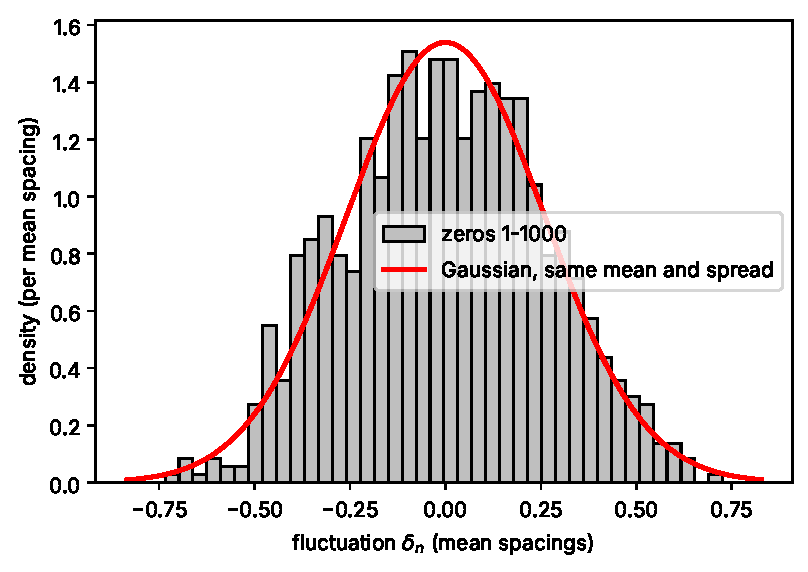
\includegraphics[width=0.85\linewidth]{figs/probability_hist_fluct.pdf}
\caption{Histogram, normalized to a density by \cref{eq:probability-hist-density}, of the fluctuations $\delta_n=(t_n-s_n)/\gap_n$ of the zeta zeros $n=1$--$1000$ about their smooth positions $s_n$, measured in local mean spacings $\gap_n$. The red curve is a Gaussian with the same mean and spread $\sigma_x$. The fluctuations are confined to a few tenths of a mean spacing.}
\label{fig:probability-hist_fluct}
\end{figure}

\begin{keyideas}

\item Variance is the expected squared deviation from the mean; $\sigma^2=E[X^2]-\mu^2$, \cref{eq:probability-var-shortcut}; $\mathrm{Var}(aX+b)=a^2\sigma^2$, \cref{eq:probability-var-scale}.
\item For a list, $\sigma_x$ divides by $n$ and $\hat\sigma$ by $n-1$; both measure spread.
\item The rms of errors combines bias and scatter: $\rms(e)^2=\bar e^{\,2}+\sigma_e^2$, \cref{eq:probability-rms-bias-spread}. It is the right score for prediction error.
\item A histogram becomes comparable with a density after dividing counts by $n\Delta$, \cref{eq:probability-hist-density}.

\end{keyideas}

%====================================================================
\section{Two distributions you must know}\label{sec:probability-gauss-exp}
% DYK-BEGIN
\begin{didyouknow}{Death by Horse Kick}
In 1898 Ladislaus Bortkiewicz showed that the yearly number of Prussian cavalrymen killed by horse kicks, recorded across army corps over 20 years, closely followed a Poisson distribution. Rare, independent events spread over many opportunities produce Poisson counts, whatever their cause. His book, \emph{The Law of Small Numbers}, made this grim dataset one of the most famous examples in statistics.
\end{didyouknow}
% DYK-END

\subsection{The Gaussian}

The \emph{Gaussian} (or \emph{normal}) density with mean $\mu$ and standard deviation $\sigma$ is
\begin{equation}
f(x) = \frac{1}{\sigma\sqrt{2\pi}}\exp\!\Bigl[-\frac{(x-\mu)^2}{2\sigma^2}\Bigr].
\label{eq:probability-gauss}
\end{equation}
It is the bell curve: symmetric about $\mu$, falling off faster than any power of $x$. With the substitution $u=(x-\mu)/\sigma$ (so $\dd x=\sigma\,\dd u$) every Gaussian becomes the \emph{standard normal} density
\begin{equation}
\varphi(u) = \frac{1}{\sqrt{2\pi}}e^{-u^2/2},
\label{eq:probability-stdnormal}
\end{equation}
because $f(x)\,\dd x = \frac{1}{\sigma\sqrt{2\pi}}e^{-u^2/2}\,\sigma\,\dd u = \varphi(u)\,\dd u$. The variable $u$ is called the \emph{z-score}: it measures distance from the mean in units of $\sigma$.

\begin{beyond}
\textbf{Taken on trust: the normalization $\int_{-\infty}^{\infty}e^{-u^2/2}\,\dd u=\sqrt{2\pi}$.} There is no elementary antiderivative of $e^{-u^2/2}$, so this needs a trick that uses integrals over a plane, which this book does not develop. The idea: call the integral $I$. Then $I^2$ is the integral of $e^{-(u^2+v^2)/2}$ over the whole $(u,v)$ plane. The integrand depends only on the distance $r=\sqrt{u^2+v^2}$ from the origin, so slice the plane into thin rings of radius $r$, width $\dd r$ and area $2\pi r\,\dd r$. Then $I^2=\int_0^\infty e^{-r^2/2}\,2\pi r\,\dd r = 2\pi\bigl[-e^{-r^2/2}\bigr]_0^\infty=2\pi$. The careful version of this argument is in \cite{rhb}.
\end{beyond}

Given the normalization, the mean and variance follow by calculus you know.

\paragraph{Mean.} Using $u=(x-\mu)/\sigma$, so $x=\mu+\sigma u$,
\begin{align*}
E[X] &= \int_{-\infty}^{\infty}(\mu+\sigma u)\,\varphi(u)\,\dd u\\
&= \mu\int_{-\infty}^{\infty}\varphi(u)\,\dd u + \frac{\sigma}{\sqrt{2\pi}}\int_{-\infty}^{\infty}u\,e^{-u^2/2}\,\dd u\\
&= \mu\cdot1 + \frac{\sigma}{\sqrt{2\pi}}\Bigl[-e^{-u^2/2}\Bigr]_{-\infty}^{\infty} \quad\text{(antiderivative of $ue^{-u^2/2}$)}\\
&= \mu + 0 = \mu .
\end{align*}

\paragraph{Variance.} $\mathrm{Var}(X)=E[(X-\mu)^2]=\sigma^2\int u^2\varphi(u)\,\dd u$. Integrate by parts, writing $u^2e^{-u^2/2}=u\cdot\bigl(ue^{-u^2/2}\bigr)$ and using $\int ue^{-u^2/2}\,\dd u=-e^{-u^2/2}$:
\begin{align*}
\int_{-\infty}^{\infty}u^2e^{-u^2/2}\,\dd u &= \Bigl[u\cdot\bigl(-e^{-u^2/2}\bigr)\Bigr]_{-\infty}^{\infty} - \int_{-\infty}^{\infty}1\cdot\bigl(-e^{-u^2/2}\bigr)\,\dd u\\
&= 0 + \sqrt{2\pi} \quad\text{($ue^{-u^2/2}\to0$ at $\pm\infty$; normalization)}.
\end{align*}
Dividing by $\sqrt{2\pi}$ gives $\int u^2\varphi\,\dd u=1$, so $\mathrm{Var}(X)=\sigma^2$. The parameters $\mu$ and $\sigma$ in \cref{eq:probability-gauss} really are the mean and standard deviation.

\paragraph{Tail probabilities.} The probability of landing within $k$ standard deviations of the mean, $P(\abs{X-\mu}<k\sigma)=\int_{-k}^{k}\varphi(u)\,\dd u$, has no elementary closed form; it is tabulated, or computed in Python as \texttt{scipy.special.erf(k/np.sqrt(2))}. The standard values are
\begin{equation}
P(\abs{u}<1)=0.6827,\qquad P(\abs{u}<2)=0.9545,\qquad P(\abs{u}<3)=0.9973,\qquad P(\abs{u}<1.960)=0.9500 .
\label{eq:probability-gauss-table}
\end{equation}
The last entry is why ``$\pm1.96\,\sigma$'' appears in 95\% intervals (\cref{sec:probability-sampling}). \Cref{fig:probability-gaussian} shows the first two.

\begin{figure}[htbp]\centering
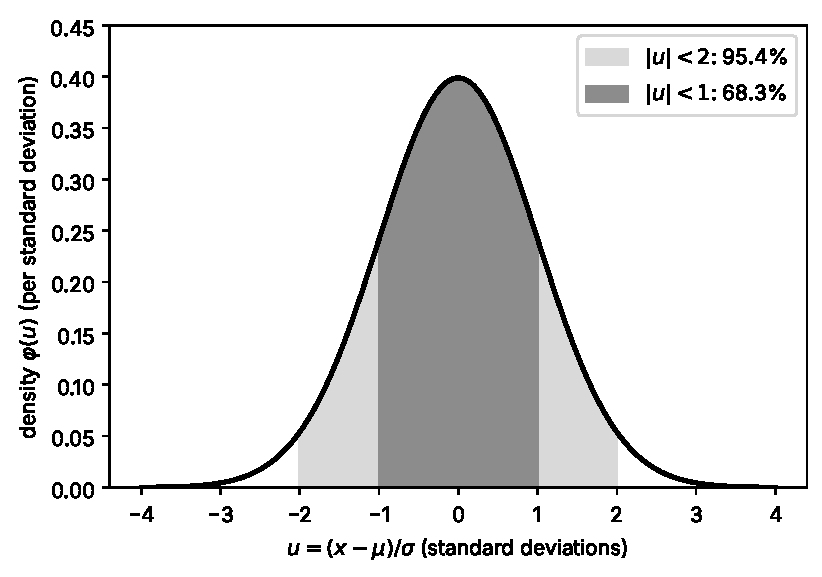
\includegraphics[width=0.85\linewidth]{figs/probability_gaussian.pdf}
\caption{The standard normal density $\varphi(u)$ of \cref{eq:probability-stdnormal}. The dark band $\abs{u}<1$ holds 68.3\% of the probability; together with the light bands, $\abs{u}<2$ holds 95.4\%. A Gaussian with any $\mu$ and $\sigma$ looks the same with $u=(x-\mu)/\sigma$ on the horizontal axis.}
\label{fig:probability-gaussian}
\end{figure}

Why does the Gaussian appear so often? The reason is a theorem about sums of many independent random contributions, which we state in \cref{sec:probability-sampling} (the central limit theorem). Measurement errors that are the sum of many small independent disturbances tend to be Gaussian; that is a tendency, not a law, and \cref{fig:probability-hist_fluct} should be read as a comparison, not as a claim that the zeros' fluctuations are exactly Gaussian.

\begin{pitfall}
The rule ``95\% within $1.96\,\sigma$'' is a property of the Gaussian. For other distributions the fraction can be very different. The only guarantee valid for \emph{every} distribution with finite variance is the much weaker Chebyshev bound, proved later in this chapter (\cref{sec:probability-sampling}): at least 75\% within $2\sigma$.
\end{pitfall}

\subsection{The exponential distribution and the Poisson process}

Now a distribution that you can derive from a physical picture. Imagine points scattered along a line ``completely at random'': clicks of a Geiger counter in time, raindrops landing along a gutter. Make three assumptions, which together define a \emph{Poisson process} of unit rate:
\begin{enumerate}
\item the probability of a point in any tiny interval of length $\dd s$ is $\dd s$ (so the mean density of points is 1 per unit length, and the mean gap is 1);
\item the probability of two or more points in a tiny interval is negligible compared with $\dd s$;
\item what happens in non-overlapping intervals is independent: knowing where the points are in one interval tells you nothing about any other.
\end{enumerate}
Assumption 3 is the heart of it: the points know nothing about one another. ``Independent'' will be defined precisely in \cref{sec:probability-correlation}; for now it means that probabilities of events in different intervals multiply.

\paragraph{Probability of an empty interval.} What is the probability $P_0(s)$ that an interval of length $s$ contains no point? Split it into $n$ equal pieces of length $s/n$. For large $n$ each piece contains a point with probability $s/n$ (assumption 1) and is empty with probability $1-s/n$. By assumption 3 the pieces are independent, so the probability that all $n$ are empty is the product
\[
P_0(s) \approx \Bigl(1-\frac sn\Bigr)^n .
\]
The approximation comes from assumptions 1 and 2 holding only for tiny pieces. Precisely, each piece is empty with probability $1-s/n+\epsilon_n$, where assumptions 1 and 2 say only that $\epsilon_n$ is negligible compared with $1/n$, that is, $n\epsilon_n\to0$. We show below that $n\log(1-x)\to-s$ for $x=s/n$; the argument uses only that $nx\to s$ and $x\to0$, and $x=s/n-\epsilon_n$ satisfies both. So the small errors $\epsilon_n$ do not accumulate over the $n$ pieces, and the approximation becomes exact as $n\to\infty$. To find the limit take the logarithm and use the Taylor series $\log(1-x)=-\sum_{j\ge1}x^j/j$ from Chapter~\ref{ch:series}, valid for $0\le x<1$, with $x=s/n$:
\begin{align*}
n\log\Bigl(1-\frac sn\Bigr) &= -n\sum_{j=1}^{\infty}\frac{(s/n)^j}{j}\\
&= -s - n\sum_{j=2}^{\infty}\frac{(s/n)^j}{j} \quad\text{(separate the $j=1$ term)}.
\end{align*}
The remainder is small. Each term obeys $(s/n)^j/j\le (s/n)^j$, so by the geometric series (Chapter~\ref{ch:series}), for $n>s$,
\[
0\le n\sum_{j=2}^{\infty}\frac{(s/n)^j}{j} \le n\,\frac{(s/n)^2}{1-s/n} = \frac{s^2}{n-s}\;\longrightarrow\;0 \quad (n\to\infty).
\]
Hence $n\log(1-s/n)\to -s$, and since the exponential function is continuous,
\begin{equation}
P_0(s) = \lim_{n\to\infty}\Bigl(1-\frac sn\Bigr)^n = e^{-s}.
\label{eq:probability-empty}
\end{equation}
\Cref{tab:probability-limit} shows how quickly the limit is approached for $s=1$.

\begin{table}[htbp]\centering
\caption{Approach of $(1-1/n)^n$ to $e^{-1}$, the probability that an interval of one mean gap in a Poisson process is empty.}
\label{tab:probability-limit}
\begin{tabular}{lcccc}
\toprule
$n$ & 10 & 100 & 1000 & $\infty$ \\
\midrule
$(1-1/n)^n$ & 0.348678 & 0.366032 & 0.367695 & $e^{-1}=0.367879$\\
\bottomrule
\end{tabular}
\end{table}

\paragraph{The gap distribution.} Stand on one point of the process and look forward. The next point lies farther than $s$ exactly when the interval of length $s$ ahead of you is empty. By assumption 3 the interval ahead does not care that a point sits where you stand, so $P(\text{gap}>s)=e^{-s}$, and the CDF of the gap is $F(s)=P(\text{gap}\le s)=1-e^{-s}$ for $s\ge0$. Differentiating, the gap density is
\begin{equation}
p(s) = F'(s) = e^{-s}\qquad (s\ge0).
\label{eq:probability-exponential}
\end{equation}
This is the \emph{exponential distribution}, and it is the Poisson law plotted in the paper's Fig.~2.

\paragraph{Mean and variance.} Integration by parts gives
\[
E[s]=\int_0^\infty s\,e^{-s}\,\dd s = \bigl[-se^{-s}\bigr]_0^\infty+\int_0^\infty e^{-s}\,\dd s = 0+1 = 1,
\]
as it must, since the rate was 1. Once more by parts, $E[s^2]=\int_0^\infty s^2e^{-s}\,\dd s=\bigl[-s^2e^{-s}\bigr]_0^\infty+2\int_0^\infty se^{-s}\,\dd s=2$, so $\mathrm{Var}(s)=2-1^2=1$.

Look at the shape of \cref{eq:probability-exponential}: it is largest at $s=0$. In a Poisson process the most likely gap is no gap at all; points that ignore each other often land almost on top of each other. The zeta zeros do the opposite. \Cref{fig:probability-exponential} compares the gaps of a simulated Poisson process with the \emph{unfolded} spacings of the first $10^4$ zeros (spacings rescaled to have mean 1; Chapter~\ref{ch:counting-zeros}). The zeros almost never come close together: they repel. Chapter~\ref{ch:level-statistics} derives the curve the zeros do follow.

\begin{figure}[htbp]\centering
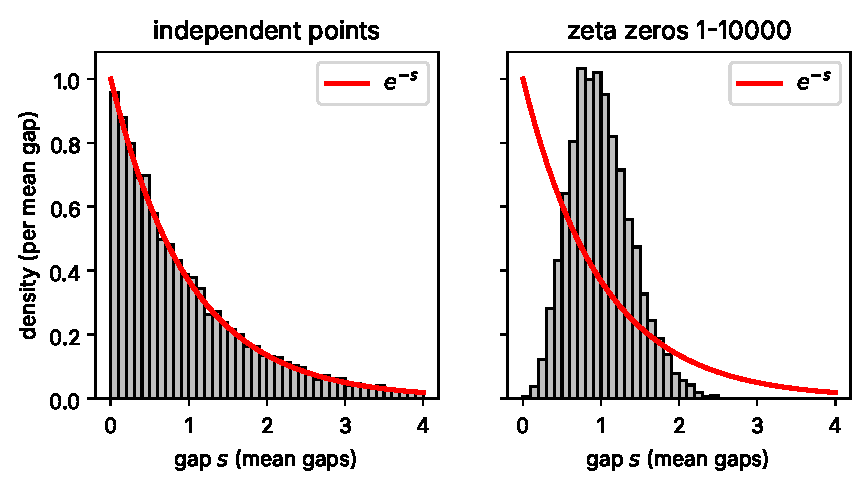
\includegraphics[width=0.85\linewidth]{figs/probability_exponential.pdf}
\caption{Left: gaps between $10^4$ points dropped independently and uniformly on an interval of length $10^4$ (seed 1; for $10^4$ points this is indistinguishable in practice from a unit-rate Poisson process, although strictly a Poisson process has a random number of points), against the exponential law $e^{-s}$ of \cref{eq:probability-exponential}. Right: unfolded spacings of the first $10^4$ zeta zeros against the same law. Small gaps are the most common for independent points but are strongly suppressed for the zeros.}
\label{fig:probability-exponential}
\end{figure}

\begin{sample}{Gap probabilities in a Poisson process}
For a unit-rate Poisson process, find (a) the probability that a gap is shorter than 0.1 mean gaps, (b) the probability that it is longer than 2 mean gaps, (c) the median gap.

\textbf{Step 1: Small gaps.} $P(\text{gap}<0.1)=F(0.1)=1-e^{-0.1}=1-0.904837=0.095163$.

\textbf{Step 2: Long gaps.} $P(\text{gap}>2)=e^{-2}=0.135335$.

\textbf{Step 3: Median.} The median $m$ splits the probability in half: $F(m)=\tfrac12$, so $e^{-m}=\tfrac12$ and $m=\log2=0.693147$.
\[
\boxed{(a)\ 0.0952,\quad (b)\ 0.1353,\quad (c)\ \log 2\approx0.693}
\]
Nearly one gap in ten is shorter than a tenth of the mean. The median is below the mean 1 because the long tail pulls the mean upward.
\end{sample}

\begin{checkpoint}
For an exponential gap distribution, where is the density largest? What does that say about the zeros, whose spacing histogram in \cref{fig:probability-exponential} is near zero at $s=0$?
\end{checkpoint}
\checkanswer{At $s=0$, since $e^{-s}$ decreases. Uncorrelated points cluster. A histogram that vanishes at $s=0$ shows that the zeros are not independent: they avoid each other (level repulsion, Chapter~\ref{ch:level-statistics}).}

\begin{keyideas}

\item The Gaussian \cref{eq:probability-gauss} has mean $\mu$ and variance $\sigma^2$; 68.3\% of probability lies within $1\sigma$, 95\% within $1.96\sigma$, \cref{eq:probability-gauss-table}.
\item Independent points of unit density leave empty intervals of length $s$ with probability $e^{-s}$, \cref{eq:probability-empty}; their gaps are exponentially distributed with mean 1 and variance 1, \cref{eq:probability-exponential}.
\item The zeta zeros are not like independent points: their small spacings are suppressed.

\end{keyideas}

%====================================================================
\section{Covariance and correlation}\label{sec:probability-correlation}

\subsection{Two random variables at once}

Often two quantities are measured together: height and weight, the true and the predicted position of a zero. Their \emph{joint distribution} for discrete variables is the list $p(x_j,y_k)=P(X=x_j\text{ and }Y=y_k)$. Summing over all values of $Y$ recovers the distribution of $X$ alone, $p_X(x_j)=\sum_k p(x_j,y_k)$, because the events ``$Y=y_k$'' are mutually exclusive and exhaust all possibilities; similarly for $p_Y$.

\paragraph{Expectation of a sum.} For any function $g(x,y)$, $E[g(X,Y)]=\sum_{j,k}g(x_j,y_k)\,p(x_j,y_k)$. With $g=x+y$:
\begin{align*}
E[X+Y] &= \sum_{j,k}(x_j+y_k)\,p(x_j,y_k)\\
&= \sum_j x_j\sum_k p(x_j,y_k) + \sum_k y_k\sum_j p(x_j,y_k) \quad\text{(split, reorder)}\\
&= \sum_j x_j\,p_X(x_j)+\sum_k y_k\,p_Y(y_k) = E[X]+E[Y].
\end{align*}
This holds for \emph{any} two random variables, related or not.

\paragraph{Independence.} $X$ and $Y$ are \emph{independent} if $p(x_j,y_k)=p_X(x_j)\,p_Y(y_k)$ for all $j,k$: knowing one tells you nothing about the other. Then
\begin{equation}
E[XY]=\sum_{j,k}x_jy_k\,p_X(x_j)p_Y(y_k) = \Bigl(\sum_j x_jp_X(x_j)\Bigr)\Bigl(\sum_ky_kp_Y(y_k)\Bigr)=E[X]\,E[Y].
\label{eq:probability-indep-product}
\end{equation}
\begin{beyond}
\textbf{Taken on trust: continuous pairs.} For two continuous variables the joint distribution is a \emph{joint density} $f(x,y)$, and probabilities of rectangles are iterated integrals, $P(a<X<b\text{ and }c<Y<d)=\int_a^b\Bigl[\int_c^d f(x,y)\,\dd y\Bigr]\dd x$: first integrate over $y$ with $x$ held fixed, then integrate the result over $x$. Sums over $j$ and $k$ become such integrals, the density of $X$ alone is $f_X(x)=\int f(x,y)\,\dd y$, and independence means $f(x,y)=f_X(x)f_Y(y)$. With these replacements every result of this section holds by the same steps; the justification that iterated integrals may be split and reordered like sums is in \cite{rhb}. We use the continuous results only in the same form as the discrete ones.
\end{beyond}

\subsection{Covariance}

The \emph{covariance} measures whether two variables tend to be above their means together:
\begin{equation}
\mathrm{Cov}(X,Y)=E\bigl[(X-\mu_X)(Y-\mu_Y)\bigr] = E[XY]-\mu_X\mu_Y .
\label{eq:probability-cov}
\end{equation}
The second form follows by expanding the product and using linearity, exactly as in \cref{eq:probability-var-shortcut}. Note $\mathrm{Cov}(X,X)=\mathrm{Var}(X)$. By \cref{eq:probability-indep-product}, independent variables have zero covariance. (The converse is false: zero covariance does not imply independence; Problem~28.)

The variance of a sum follows. Write $X'=X-\mu_X$, $Y'=Y-\mu_Y$; the sum $X+Y$ has mean $\mu_X+\mu_Y$, so
\begin{align}
\mathrm{Var}(X+Y) &= E\bigl[(X'+Y')^2\bigr] = E[X'^2]+2E[X'Y']+E[Y'^2]\nonumber\\
&= \mathrm{Var}(X)+\mathrm{Var}(Y)+2\,\mathrm{Cov}(X,Y).
\label{eq:probability-var-sum}
\end{align}
For independent variables the covariance term vanishes and variances simply add. This one fact drives the whole of \cref{sec:probability-sampling}.

\paragraph{Correlation coefficient of two random variables.} For random variables with $\sigma_X>0$ and $\sigma_Y>0$, the \emph{correlation coefficient} is
\begin{equation}
\rho=\frac{\mathrm{Cov}(X,Y)}{\sigma_X\sigma_Y}.
\label{eq:probability-rho}
\end{equation}
For the empirical distribution of two paired lists (each pair $(x_i,y_i)$ picked with probability $1/n$), $\mathrm{Cov}$ becomes the list covariance and $\rho$ becomes the Pearson coefficient $r$ defined below. The proof of $\abs{r}\le1$ given below also proves $\abs{\rho}\le1$: replace $\sum u_iv_i$ by $E[X'Y']$, $\sum u_i^2$ by $E[X'^2]$ and $\sum v_i^2$ by $E[Y'^2]$; the proof uses only that the expectation of a square is nonnegative and that expectation is linear.

\subsection{The Pearson correlation coefficient}

Covariance has awkward units (units of $X$ times units of $Y$) and changes if you rescale either variable. Dividing by the two standard deviations removes both defects. For two lists $x_1,\dots,x_n$ and $y_1,\dots,y_n$, the \emph{Pearson correlation coefficient} is
\begin{equation}
\corr(x,y) = r = \frac{\sum_{i=1}^n (x_i-\bar x)(y_i-\bar y)}{\sqrt{\sum_{i=1}^n (x_i-\bar x)^2}\,\sqrt{\sum_{i=1}^n (y_i-\bar y)^2}} .
\label{eq:probability-pearson}
\end{equation}
If you divide numerator and denominator by $n$, the numerator is the list covariance $c_{xy}=\frac1n\sum(x_i-\bar x)(y_i-\bar y)$ and the denominator is $\sigma_x\sigma_y$, so $r=c_{xy}/(\sigma_x\sigma_y)$. The factors of $n$ (or $n-1$) cancel, so it does not matter which convention you use for the spreads, provided you use the same one top and bottom.

\paragraph{A geometric reading.} Define the \emph{centered} lists $u_i=x_i-\bar x$ and $v_i=y_i-\bar y$, and think of them as vectors with $n$ components. The numerator of \cref{eq:probability-pearson} is their dot product $\mathbf u\cdot\mathbf v=\sum u_iv_i$; the denominator is the product of their lengths. In three dimensions you know that $\mathbf u\cdot\mathbf v=\abs{\mathbf u}\abs{\mathbf v}\cos\theta$, so $r$ is the cosine of the angle between the centered data vectors. That already suggests $-1\le r\le1$. In $n$ dimensions we need a proof.

\subsection{Why $-1\le r\le1$: the Cauchy--Schwarz inequality}

\textbf{Theorem (Cauchy--Schwarz, proved).} For any real lists $u_1,\dots,u_n$ and $v_1,\dots,v_n$,
\begin{equation}
\Bigl(\sum_{i=1}^n u_iv_i\Bigr)^2 \le \Bigl(\sum_{i=1}^n u_i^2\Bigr)\Bigl(\sum_{i=1}^n v_i^2\Bigr),
\label{eq:probability-cs}
\end{equation}
with equality if and only if one list is a constant multiple of the other.

\emph{Proof.} If every $v_i=0$ both sides are zero and there is nothing to prove; so suppose $\sum v_i^2>0$. For any real number $\lambda$, a sum of squares is never negative:
\begin{align*}
0 \le g(\lambda) &= \sum_{i=1}^n (u_i-\lambda v_i)^2\\
&= \sum u_i^2 - 2\lambda\sum u_iv_i + \lambda^2\sum v_i^2 \quad\text{(expand the square)}.
\end{align*}
The inequality $g(\lambda)\ge0$ holds for every $\lambda$, so we may pick the most useful one, the $\lambda$ at which $g$ is smallest. Setting the derivative to zero, $g'(\lambda)=-2\sum u_iv_i+2\lambda\sum v_i^2=0$, gives $\lambda^*=\sum u_iv_i\big/\sum v_i^2$. (The proof uses only $g(\lambda^*)\ge0$; that $\lambda^*$ minimizes $g$ merely explains why it is the best choice.) Substituting,
\begin{align*}
0\le g(\lambda^*) &= \sum u_i^2 - 2\frac{(\sum u_iv_i)^2}{\sum v_i^2}+\frac{(\sum u_iv_i)^2}{(\sum v_i^2)^2}\sum v_i^2\\
&= \sum u_i^2 - \frac{(\sum u_iv_i)^2}{\sum v_i^2}.
\end{align*}
Multiplying by the positive number $\sum v_i^2$ gives \cref{eq:probability-cs}. Equality holds exactly when $g(\lambda^*)=0$, that is, when every term $(u_i-\lambda^*v_i)^2$ vanishes, i.e. $u_i=\lambda^*v_i$ for all $i$. \hfill$\square$

Applying \cref{eq:probability-cs} to the centered lists and taking square roots,
\[
\Bigl|\sum(x_i-\bar x)(y_i-\bar y)\Bigr| \le \sqrt{\sum(x_i-\bar x)^2}\sqrt{\sum(y_i-\bar y)^2},
\]
which is precisely $\abs{r}\le1$. So:
\begin{itemize}
\item $r=+1$ exactly when $y_i-\bar y=\lambda(x_i-\bar x)$ with $\lambda>0$: the points lie on a rising straight line;
\item $r=-1$ exactly when they lie on a falling straight line;
\item $r=0$ when there is no \emph{linear} tendency for one to rise with the other.
\end{itemize}
Note the word ``linear''. Correlation is blind to the slope's size, and blind to nonlinear relations.

\begin{sample}{Correlation by hand}
Find $r$ for $x=(1,2,3,4,5)$ and $y=(2,1,4,3,5)$.

\textbf{Step 1: Means.} $\bar x=15/5=3$ and $\bar y=15/5=3$.

\textbf{Step 2: Centered lists.} $u=(-2,-1,0,1,2)$ and $v=(-1,-2,1,0,2)$.

\textbf{Step 3: Sums.} $\sum u_iv_i = 2+2+0+0+4=8$; $\sum u_i^2=4+1+0+1+4=10$; $\sum v_i^2=1+4+1+0+4=10$.

\textbf{Step 4: Coefficient.} $r=8/\sqrt{10\cdot10}=0.8$.
\[
\boxed{r=0.8}
\]
The two lists rise together but not along a perfect line.
\end{sample}

\begin{checkpoint}
You multiply every entry of a prediction $p$ by 2. What happens to $\corr(p,y)$? What if you multiply by $-2$?
\end{checkpoint}
\checkanswer{Multiplying by 2 multiplies the centered list by 2, so the numerator of \cref{eq:probability-pearson} and the factor $\sqrt{\sum(p_i-\bar p)^2}$ both double: $r$ is unchanged. Multiplying by $-2$ flips the sign of the numerator but not of the square root: $r\to-r$.}

\begin{keyideas}

\item Expectations of sums add for any variables; for independent variables $E[XY]=E[X]E[Y]$ and variances add, \cref{eq:probability-var-sum}.
\item The Pearson coefficient \cref{eq:probability-pearson} is the cosine of the angle between centered data vectors.
\item Cauchy--Schwarz \cref{eq:probability-cs} proves $-1\le r\le 1$, with $\pm1$ only for an exact linear relation.
\item Correlation ignores the size of the slope: it is unchanged by rescaling either list by a positive factor.

\end{keyideas}

%====================================================================
\section{Correlation versus rms error}\label{sec:probability-corr-rms}

\subsection{One identity that ties them together}

The paper reports both an rms error and a correlation for each prediction because they answer different questions. The rms asks: \emph{how far off is the prediction?} The correlation asks: \emph{does the prediction go up when the truth goes up?} A single identity tells us exactly how they are related.

Let $y_1,\dots,y_n$ be the true values and $p_1,\dots,p_n$ the predictions. Split each list into its mean and a centered part, $p_i=\bar p+p_i'$ and $y_i=\bar y+y_i'$, where $\sum p_i'=\sum y_i'=0$. Then
\begin{align*}
p_i-y_i &= (\bar p-\bar y) + (p_i'-y_i'),\\
(p_i-y_i)^2 &= (\bar p-\bar y)^2 + 2(\bar p-\bar y)(p_i'-y_i') + (p_i'-y_i')^2 .
\end{align*}
Average over $i$. The middle term averages to zero, because $\frac1n\sum(p_i'-y_i')=0$. The last term is $\overline{p'^2}+\overline{y'^2}-2\,\overline{p'y'}=\sigma_p^2+\sigma_y^2-2c_{py}$, where $c_{py}$ is the list covariance. Finally $c_{py}=r\,\sigma_p\sigma_y$ with $r=\corr(p,y)$. So
\begin{equation}
\rms(p-y)^2 = (\bar p-\bar y)^2 + \sigma_p^2 + \sigma_y^2 - 2r\,\sigma_p\sigma_y .
\label{eq:probability-msedecomp}
\end{equation}
This is exact: no approximation, no assumption about distributions. It is the law of cosines in disguise: if the centered vectors $\mathbf p'$ and $\mathbf y'$ make an angle $\theta$ with $\cos\theta=r$, the squared length of their difference is $\abs{\mathbf p'}^2+\abs{\mathbf y'}^2-2\abs{\mathbf p'}\abs{\mathbf y'}\cos\theta$.

\subsection{Three consequences}

Suppose, as for the fluctuations scored in the paper, that the truth has mean close to zero, $\bar y\approx0$, so that $\sigma_y\approx\rms(y)$ by \cref{eq:probability-rms-bias-spread}. The \emph{null} prediction $p=0$ has error $\rms(0-y)=\rms(y)$.

\paragraph{1. Right shape, wrong amplitude.} Let $p=a y$ with $a>0$. Then $r=+1$ (a rising straight line), yet the error is $\rms(ay-y)=\abs{a-1}\rms(y)$. A prediction can be perfectly correlated with the truth and still have a large rms. For $a=2$ the error equals the null; for $a>2$ it is \emph{worse} than predicting nothing.

\paragraph{2. Uncorrelated predictions are worse than the null.} Put $r=0$ and $\bar p=\bar y=0$ in \cref{eq:probability-msedecomp}:
\begin{equation}
\rms(p-y)^2 = \sigma_y^2+\sigma_p^2 \ \ge\ \sigma_y^2 = (\text{null})^2 .
\label{eq:probability-uncorr}
\end{equation}
A prediction that wiggles independently of the truth adds its own variance to the error. The bigger its wiggles, the worse it does. Predicting nothing is better than predicting noise.

\paragraph{3. The best possible rms at a given correlation.} Fix $r$ and $\sigma_y$ and ask which prediction minimizes \cref{eq:probability-msedecomp}. The first term is minimized (to zero) by $\bar p=\bar y$. The $\sigma_p$ terms are a quadratic, which we complete to a square:
\[
\sigma_p^2-2r\sigma_y\sigma_p = (\sigma_p-r\sigma_y)^2 - r^2\sigma_y^2 .
\]
If $r>0$, the square vanishes at $\sigma_p=r\sigma_y$, and then
\begin{equation}
\rms(p-y)_{\min} = \sigma_y\sqrt{1-r^2}\qquad(r>0).
\label{eq:probability-bestrms}
\end{equation}
If $r\le0$, the expression $\sigma_p^2-2r\sigma_y\sigma_p$ is positive for every $\sigma_p>0$ (both terms are nonnegative and the first is positive), so the rms exceeds $\sigma_y$ and only approaches $\sigma_y$ as $\sigma_p\to0$. (The value $\sigma_p=0$ itself is excluded, because there the correlation is undefined; see the pitfall below.) No prediction with nonpositive correlation beats the null. Two lessons follow. The optimal amplitude is $r$ times the true amplitude, smaller than the truth whenever the correlation is imperfect: a cautious predictor should shrink its fluctuations. And a correlation of 0.96, which sounds nearly perfect, can at best cut the error to $\sqrt{1-0.96^2}=0.28$ of the null.

\begin{sample}{Correct shape, wrong amplitude}
The true fluctuations on five levels are $y=(0.3,-0.2,0.1,-0.4,0.2)$ (in mean spacings). Compare the null with the predictions $p=0.5y$, $p=2y$ and $p=3y$.

\textbf{Step 1: Null.} $\bar y=0$. $\overline{y^2}=(0.09+0.04+0.01+0.16+0.04)/5=0.34/5=0.068$, so the null rms is $\rms(y)=\sqrt{0.068}=0.2608$.

\textbf{Step 2: Correlations.} Each $p$ is a positive multiple of $y$, so $r=+1$ in all three cases.

\textbf{Step 3: Errors.} $p-y=(a-1)y$, so $\rms(p-y)=\abs{a-1}\times0.2608$: for $a=0.5$, $0.1304$; for $a=2$, $0.2608$; for $a=3$, $0.5215$.
\[
\boxed{\text{null }0.261;\quad a=0.5:\ 0.130;\quad a=2:\ 0.261;\quad a=3:\ 0.522;\quad r=+1\text{ throughout}}
\]
The $a=3$ prediction is perfectly correlated with the truth and twice as bad as the null. Correlation and rms are not interchangeable scores.
\end{sample}

\begin{checkpoint}
A prediction has correlation $+1$ with the truth. Must it beat the null?
\end{checkpoint}
\checkanswer{No. With $p=ay$, the rms is $\abs{a-1}\rms(y)$, which exceeds the null whenever $a>2$. Correlation measures shape, rms measures size; you need both.}

\begin{sample}{How good can a prediction with correlation $r$ be?}
On the held-out zeros 401--500 the paper's null rms is $0.263$ (Table~V). The zero-parameter prime formula with the prime $2$ only has correlation $+0.66$; with 3 primes, $+0.90$; with 6 primes, $+0.96$ (Table~V). Use \cref{eq:probability-bestrms} to find the smallest rms any prediction with these correlations could have, and compare with the rms values in Table~V: 0.198, 0.116, 0.074.

\textbf{Step 1: Assumption.} Take $\sigma_y\approx0.263$. This holds if the true fluctuations on the holdout have mean close to zero; if their mean were not small, $\sigma_y$ would be below 0.263 and the bound below would be lower.

\textbf{Step 2: The prime 2.} $\sqrt{1-0.66^2}=\sqrt{0.5644}=0.7513$; bound $0.263\times0.7513=0.1976$.

\textbf{Step 3: Three primes.} $\sqrt{1-0.81}=\sqrt{0.19}=0.4359$; bound $0.1146$.

\textbf{Step 4: Six primes.} $\sqrt{1-0.9216}=\sqrt{0.0784}=0.28$; bound $0.0736$.
\[
\boxed{\text{bounds } 0.198,\ 0.115,\ 0.074 \ \text{ vs. Table V } 0.198,\ 0.116,\ 0.074}
\]
The formula, which has no fitted parameters at all, sits essentially on the bound: its fluctuations have nearly the optimal amplitude for its correlation. One caution: the correlations are rounded to two digits, and near $r=1$ the bound is very sensitive to rounding. For the 25-prime column ($r=+0.99$, rms 0.043) the bound with $r=0.99$ is $0.037$, but with $r=0.985$, which also rounds to 0.99, it is $0.045$. So no conclusion should be drawn from the last column's comparison.
\end{sample}

\Cref{fig:probability-corr_rms} shows the two extremes graphically, using the prime-2 wave of Running Example RE2 as the ``truth''.

\begin{figure}[htbp]\centering
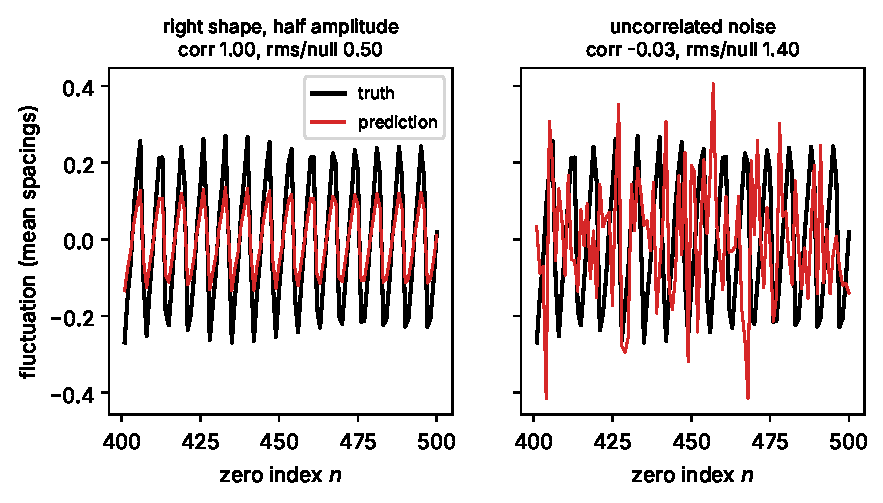
\includegraphics[width=0.85\linewidth]{figs/probability_corr_rms.pdf}
\caption{Two ways to miss. Truth (black): the prime-2 wave RE2, $-\frac1\pi\sum_{m=1}^{3}\sin(mt\log2)/(m2^{m/2})$, evaluated at the smooth zeros $s_n$, $n=401$--$500$. Left: a prediction with the right shape and half the amplitude; correlation $+1$, rms error exactly half the null. Right: Gaussian noise with the same spread as the truth (seed 2); correlation near zero, rms error close to $\sqrt2$ times the null, as \cref{eq:probability-uncorr} predicts.}
\label{fig:probability-corr_rms}
\end{figure}

\begin{pitfall}
The correlation of the null prediction is undefined. If $p_i=0$ for every $i$, the factor $\sqrt{\sum(p_i-\bar p)^2}$ in \cref{eq:probability-pearson} is zero and $r$ is $0/0$. Consistently, the paper's tables give a null rms but no null correlation. \texttt{numpy.corrcoef} returns \texttt{nan} (with a warning) in this case.
\end{pitfall}

\begin{keyideas}

\item The exact identity \cref{eq:probability-msedecomp} expresses mean-square error through means, spreads and correlation.
\item Correct shape with wrong amplitude gives $r=+1$ but rms $\abs{a-1}\rms(y)$.
\item For zero-mean truth, an uncorrelated prediction is worse than the null by its own variance, \cref{eq:probability-uncorr}.
\item At correlation $r>0$ the smallest possible rms is $\sigma_y\sqrt{1-r^2}$, reached by shrinking the prediction to amplitude $r\sigma_y$, \cref{eq:probability-bestrms}.

\end{keyideas}

%====================================================================
\section{Autocorrelation of a sequence}\label{sec:probability-autocorr}
% DYK-BEGIN
\begin{didyouknow}{Sunspots and Memory}
In 1927 the statistician George Udny Yule modeled yearly sunspot numbers by letting each year's value depend on the previous two years plus random shocks. This was the first autoregressive model, and it showed how a correlated random sequence can mimic periodic behavior. Autocorrelation measures how strongly a sequence remembers its own past, and it is the tool for telling real rhythms from noise.
\end{didyouknow}
% DYK-END

\subsection{Definition}

So far the order of a list did not matter: shuffling $x_1,\dots,x_n$ leaves $\bar x$, $\sigma_x$ and $\rms(x)$ unchanged. But the zeros come in order, and their fluctuations are not shuffled at random: neighbors are related. \emph{Autocorrelation} measures how a sequence relates to a shifted copy of itself. The sample autocorrelation at lag $k$ is
\begin{equation}
r_k = \frac{\sum_{i=1}^{n-k}(x_i-\bar x)(x_{i+k}-\bar x)}{\sum_{i=1}^{n}(x_i-\bar x)^2},\qquad k=0,1,2,\dots
\label{eq:probability-acf}
\end{equation}
It is the Pearson correlation of the sequence with itself shifted by $k$ places, with the convention that the overall mean and the full sum of squares are used for normalization. Then $r_0=1$, and $\abs{r_k}\le1$ follows from Cauchy--Schwarz (Problem~29). A positive $r_1$ says ``if this entry is above average, the next tends to be above average too''; a negative $r_1$ says ``highs tend to be followed by lows''.

Autocorrelation is most useful when the sequence is (at least roughly) \emph{stationary}: its statistical behavior does not depend on where in the sequence you look, so the relation between $x_i$ and $x_{i+k}$ depends on $k$ but not on $i$. For the zeros' fluctuations this is an approximation (their amplitude grows slowly with height, Sec.~II C of the paper); over a window of a few hundred zeros it is reasonable.

\begin{sample}{An alternating sequence}
Compute $r_1$ and $r_2$ for $x=(1,-1,1,-1,1,-1)$.

\textbf{Step 1: Mean and denominator.} $\bar x=0$; $\sum x_i^2=6$.

\textbf{Step 2: Lag 1.} The products $x_ix_{i+1}$ for $i=1,\dots,5$ are all $-1$; their sum is $-5$. So $r_1=-5/6$.

\textbf{Step 3: Lag 2.} The products $x_ix_{i+2}$ for $i=1,\dots,4$ are all $+1$; sum $4$. So $r_2=4/6$.
\[
\boxed{r_1=-0.833,\quad r_2=+0.667}
\]
The magnitudes are below 1 only because fewer pairs ($n-k$) enter the numerator than terms ($n$) enter the denominator; for a long alternating sequence $r_1\to-1$ and $r_2\to+1$.
\end{sample}

\subsection{The autocorrelation of a sinusoid}

Take $y(t)=a\sin(\omega t+\phi)$. To see what \cref{eq:probability-acf} measures for such a signal, consider first the idealized case of samples at many closely and evenly spaced times $t_i$ over a window of many periods. Then each sum in \cref{eq:probability-acf}, divided by its number of terms, is a Riemann sum for a time average, and a lag of $k$ samples is a fixed time shift $\tau$. This is an approximation: it neglects the discreteness of the sampling and the incomplete period at the ends of the window, both of which become negligible as the sampling gets finer and the window longer. Because an average over many whole periods equals the average over one period $P=2\pi/\omega$, we compute averages over one period. First, the mean is zero, because $\int_0^P\sin(\omega t+\phi)\,\dd t=0$. Next, by the identity $\sin A\sin B=\tfrac12[\cos(A-B)-\cos(A+B)]$ with $A=\omega t+\phi$ and $B=\omega t+\omega\tau+\phi$,
\[
y(t)\,y(t+\tau) = \frac{a^2}{2}\bigl[\cos(\omega\tau) - \cos(2\omega t+\omega\tau+2\phi)\bigr].
\]
The second cosine completes two full cycles in one period, so it averages to zero; the first does not depend on $t$. Therefore
\begin{equation}
\langle y(t)\,y(t+\tau)\rangle = \frac{a^2}{2}\cos(\omega\tau),
\label{eq:probability-sin-acf}
\end{equation}
where $\langle\cdot\rangle$ denotes the average over a period. Setting $\tau=0$ gives the mean square $a^2/2$, so $\rms(y)=a/\sqrt2$: this is the $\sqrt2$ of AC circuits. Dividing \cref{eq:probability-sin-acf} by its value at $\tau=0$, the autocorrelation of a sinusoid at lag $\tau$ is $\cos(\omega\tau)$: it oscillates with the same period as the signal and never dies out. When the signal is sampled instead at the smooth zeros $s_n$, as in \cref{fig:probability-autocorr}, a lag of $k$ levels corresponds to a time shift $\tau\approx k$ times the local mean spacing (defined in \cref{sec:probability-paper}), which changes slowly with height. Over a window where that spacing is nearly constant, the lag-in-levels autocorrelation still oscillates like $\cos(\omega\tau)$, but only approximately.

The same tools give the mean square of a sum of sinusoids whose frequencies are $\omega,2\omega,3\omega,\dots$. For positive integers $m\neq m'$, the identity above turns $\sin(m\omega t)\sin(m'\omega t)$ into $\tfrac12[\cos((m-m')\omega t)-\cos((m+m')\omega t)]$; both cosines complete a whole number of cycles in the period $P$ and average to zero. Cross terms vanish, and
\begin{equation}
\Bigl\langle \Bigl(\sum_m a_m\sin(m\omega t)\Bigr)^2\Bigr\rangle = \sum_m\frac{a_m^2}{2}.
\label{eq:probability-sum-ms}
\end{equation}
(When the frequencies are not integer multiples of one common $\omega$ there is no common period, but the cross terms still average to zero over a long window; this is the long-window orthogonality of sinusoids with different frequencies treated in Chapter~\ref{ch:fourier-series}. We do not need it here, because the frequencies of RE2 below are harmonics.)

\begin{sample}{The rms of the prime-2 wave (RE2)}
Running Example RE2 is $y(t)=-\frac1\pi\sum_{m=1}^{3}\frac{\sin(mt\log2)}{m\,2^{m/2}}$. Find its long-run rms.

\textbf{Step 1: Amplitudes.} $a_m=1/(\pi m 2^{m/2})$ (the overall minus sign does not affect squares):
$a_1=1/(\pi\sqrt2)=0.225079$, $a_2=1/(4\pi)=0.079577$, $a_3=1/(6\sqrt2\,\pi)=0.037513$.

\textbf{Step 2: Mean square.} The frequencies are $\omega,2\omega,3\omega$ with $\omega=\log 2$, so \cref{eq:probability-sum-ms} applies:
\[
\overline{y^2}=\tfrac12(0.050661+0.006333+0.001407)=\tfrac12(0.058400)=0.029200 .
\]
\textbf{Step 3: Root.} $\rms(y)=\sqrt{0.029200}=0.17088$.
\[
\boxed{\rms(\text{RE2})\approx0.1709}
\]
The paper's arithmetic-continuation probe uses this wave (with the opposite sign, since a level shift is minus the counting fluctuation; the rms is unaffected) as a synthetic target, sampled at the smooth zeros $401$--$500$, and records the rms of predicting no fluctuation as the ``probe-null'' $0.1708$ (App.~A, ``Key anchors''). The window covers about 15 periods of the wave, and the long-run value $0.1709$ agrees closely with the paper's $0.1708$. Evaluating the wave directly at the 100 smooth zeros 401--500 with qmnt, \texttt{qmnt.rms(qmnt.Nfl(qmnt.smooth\_zeros(n), [2]))}, reproduces the paper's $0.1708$ to within $0.001$. A small difference from the long-run value is to be expected, because on the holdout the wave is sampled at 100 discrete, unevenly spaced points rather than averaged continuously.
\end{sample}

\subsection{Predicting a value from its neighbors}

Autocorrelation decides whether you can predict a missing entry from its neighbors. Suppose a stationary sequence has mean zero, variance $\sigma^2$, lag-1 autocorrelation $\rho_1$ and lag-2 autocorrelation $\rho_2$, meaning $E[x_ix_{i\pm1}]=\rho_1\sigma^2$ and $E[x_{i-1}x_{i+1}]=\rho_2\sigma^2$. Predict $x_i$ by the average of its two neighbors, $\hat x_i=\tfrac12(x_{i-1}+x_{i+1})$. What is the correlation between prediction and truth?

\textbf{Covariance with the truth.} By linearity, $E[x_i\hat x_i]=\tfrac12(E[x_ix_{i-1}]+E[x_ix_{i+1}])=\tfrac12(2\rho_1\sigma^2)=\rho_1\sigma^2$.

\textbf{Variance of the prediction.} By \cref{eq:probability-var-sum} and \cref{eq:probability-var-scale},
\[
\mathrm{Var}(\hat x_i)=\tfrac14\bigl[\sigma^2+\sigma^2+2\rho_2\sigma^2\bigr]=\frac{\sigma^2(1+\rho_2)}{2}.
\]
\textbf{Correlation.} Dividing the covariance by the two standard deviations, as in the correlation coefficient $\rho$ of two random variables, \cref{eq:probability-rho},
\begin{equation}
\corr(\hat x_i,x_i)=\frac{\rho_1\sigma^2}{\sigma\cdot\sigma\sqrt{(1+\rho_2)/2}}=\frac{\rho_1}{\sqrt{(1+\rho_2)/2}} .
\label{eq:probability-neighbor}
\end{equation}
The sign is the sign of $\rho_1$. If neighbors are negatively correlated, a smooth interpolation between them is anticorrelated with the truth. For example, $\rho_1=-0.3$ and $\rho_2=-0.1$ give $\corr=-0.3/\sqrt{0.45}=-0.447$. This little calculation is the mechanism the paper invokes in Sec.~III for negative held-out correlations; Chapter~\ref{ch:generalization} develops the general best linear predictor.

\Cref{fig:probability-autocorr} shows autocorrelations of two sequences: the RE2 wave sampled at the smooth zeros, which oscillates because its $m=1$ term dominates (it carries 87\% of the mean square in Step~2 of the sample problem above; the $m=2,3$ harmonics distort the shape slightly away from a pure cosine), and independent noise, which is near zero at every nonzero lag.

\begin{figure}[htbp]\centering
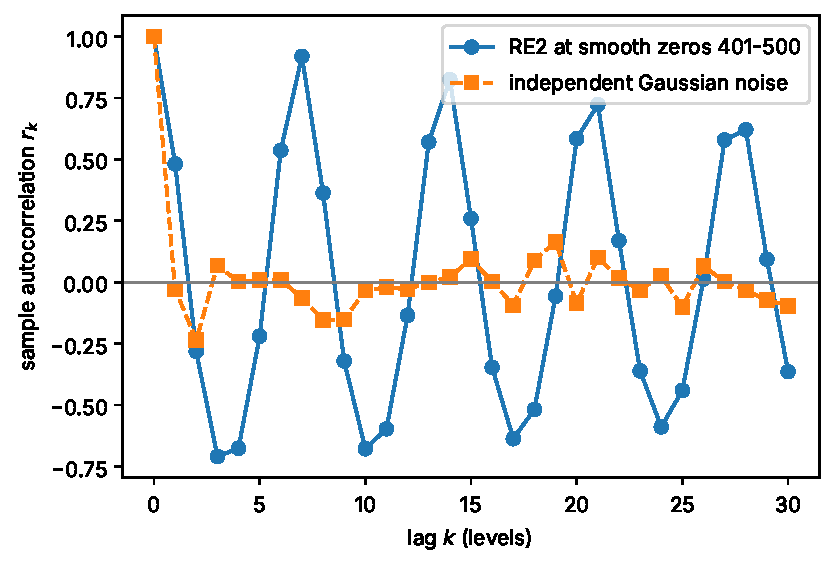
\includegraphics[width=0.85\linewidth]{figs/probability_autocorr.pdf}
\caption{Sample autocorrelation \cref{eq:probability-acf} against lag in levels. Circles: the prime-2 wave RE2 sampled at the smooth zeros $s_n$, $n=401$--$500$; it oscillates, dominated by its $m=1$ term (the $m=2,3$ harmonics modify the shape), with a period of roughly 6--7 levels, the level-count of one period $2\pi/\log 2\approx9.07$ in $t$ at these heights (compare paper Sec.~V). Squares: 100 independent Gaussian numbers (seed 1), whose autocorrelations scatter near zero.}
\label{fig:probability-autocorr}
\end{figure}

\begin{pycode}
import numpy as np

def autocorr(x, kmax):
    """Sample autocorrelation r_0..r_kmax, Eq. (acf)."""
    x = np.asarray(x, float) - np.mean(x)
    denom = np.sum(x**2)
    return np.array([np.sum(x[:len(x)-k] * x[k:]) / denom
                     for k in range(kmax + 1)])

print(autocorr([1, -1, 1, -1, 1, -1], 2))  # 1, -5/6, 4/6
\end{pycode}

\begin{keyideas}

\item The lag-$k$ autocorrelation \cref{eq:probability-acf} correlates a sequence with its own shifted copy; it captures the order information that $\bar x$ and $\sigma_x$ ignore.
\item A sinusoid has autocorrelation $\cos(\omega\tau)$ and rms $a/\sqrt2$; harmonically related sinusoids add in mean square, \cref{eq:probability-sum-ms}.
\item The long-run rms of RE2 is 0.1709, close to the paper's probe-null 0.1708.
\item Averaging neighbors predicts with correlation $\rho_1/\sqrt{(1+\rho_2)/2}$, \cref{eq:probability-neighbor}: negative if neighbors are negatively correlated.

\end{keyideas}

%====================================================================
\section{Sampling, estimators and the standard error}\label{sec:probability-sampling}

\subsection{Estimators}

In practice we want properties of a distribution (its mean $\mu$, its variance $\sigma^2$, the correlation between two quantities) but we see only a finite \emph{sample} $x_1,\dots,x_n$ drawn from it. An \emph{estimator} is a rule that turns the sample into a guess; $\bar x$ is an estimator of $\mu$. Because the sample is random, the estimator is itself a random variable: draw another sample and you get another value. Two questions matter. Is it right on average (is it \emph{unbiased}, $E[\text{estimator}]=\text{true value}$)? And how much does it scatter from sample to sample?

Throughout this section the draws are \emph{independent and identically distributed}: each $x_i$ has the same distribution, with mean $\mu$ and variance $\sigma^2$, and different draws are independent.

We need the two-variable results of \cref{sec:probability-correlation} for $n$ variables. Applying them repeatedly (first to $x_1+x_2$, then to $(x_1+x_2)+x_3$, and so on; for independent draws each partial sum is independent of the next draw) gives $E[\sum_ix_i]=\sum_iE[x_i]$ for any draws, and $\mathrm{Var}(\sum_ix_i)=\sum_i\mathrm{Var}(x_i)$ for independent ones.

\paragraph{The sample mean is unbiased.} By linearity, $E[\bar x]=\frac1n\sum_i E[x_i]=\frac1n\cdot n\mu=\mu$.

\paragraph{Its variance shrinks like $1/n$.} By \cref{eq:probability-var-scale} with $a=1/n$, and then \cref{eq:probability-var-sum} with all covariances zero (independence),
\begin{equation}
\mathrm{Var}(\bar x)=\frac{1}{n^2}\mathrm{Var}\Bigl(\sum_i x_i\Bigr)=\frac1{n^2}\sum_i\mathrm{Var}(x_i)=\frac{n\sigma^2}{n^2}=\frac{\sigma^2}{n}.
\label{eq:probability-var-mean}
\end{equation}
The standard deviation of the estimator is called its \emph{standard error}:
\begin{equation}
\mathrm{SE}(\bar x)=\frac{\sigma}{\sqrt n}\approx\frac{\hat\sigma}{\sqrt n}.
\label{eq:probability-se}
\end{equation}
The second form replaces the unknown $\sigma$ by its estimate. To halve the standard error you need four times as many data.

\paragraph{Why divide by $n-1$.} Let us compute the expectation of $Q=\sum_i(x_i-\bar x)^2$. First an algebraic rearrangement:
\begin{align*}
Q&=\sum_i x_i^2-2\bar x\sum_i x_i+n\bar x^2\\
&=\sum_i x_i^2 - 2\bar x\,(n\bar x) + n\bar x^2 \quad\text{($\sum_i x_i=n\bar x$)}\\
&=\sum_i x_i^2-n\bar x^2 .
\end{align*}
Now take expectations. By \cref{eq:probability-var-shortcut} applied to each $x_i$, $E[x_i^2]=\sigma^2+\mu^2$. By the same identity applied to $\bar x$, together with $E[\bar x]=\mu$ and \cref{eq:probability-var-mean}, $E[\bar x^2]=\sigma^2/n+\mu^2$. Hence
\[
E[Q]=n(\sigma^2+\mu^2)-n\Bigl(\frac{\sigma^2}{n}+\mu^2\Bigr)=(n-1)\sigma^2 .
\]
So $E[Q/(n-1)]=\sigma^2$: the $n-1$ version $\hat\sigma^2$ is unbiased, while $\sigma_x^2=Q/n$ is too small on average by the factor $(n-1)/n$. The reason is that $\bar x$ is computed from the same data and sits closer to them than the true $\mu$ does. (This is \emph{Bessel's correction}.) For example, for $n=2$ throws of a fair die, averaging over all 36 equally likely pairs, $Q/1$ averages to exactly $35/12$, the true variance found earlier, while $Q/2$ averages to $35/24\approx1.458$ (Problem~30).

\begin{pitfall}
Formula \cref{eq:probability-se} assumes \emph{independent} draws. If neighboring values are correlated, as the zeros' fluctuations are (\cref{sec:probability-autocorr}), the covariance terms in \cref{eq:probability-var-sum} no longer vanish and $\sigma/\sqrt n$ can be badly wrong. Chapter~\ref{ch:controls} treats this with the block bootstrap; the paper does the same in Sec.~III (``Other bases'').
\end{pitfall}

\subsection{The law of large numbers}

How sure can we be that $\bar x$ is close to $\mu$? A beautiful one-line inequality answers this for every distribution with finite variance.

\textbf{Chebyshev's inequality (proved).} For any random variable with mean $\mu$, variance $\sigma^2$, and any $a>0$,
\begin{equation}
P\bigl(\abs{X-\mu}\ge a\bigr)\le\frac{\sigma^2}{a^2}.
\label{eq:probability-chebyshev}
\end{equation}
\emph{Proof} (discrete case; the continuous case replaces sums by integrals). Start from the definition of variance and keep only the values far from the mean:
\begin{align*}
\sigma^2=\sum_j p_j(x_j-\mu)^2 &\ge \sum_{j:\,\abs{x_j-\mu}\ge a}p_j(x_j-\mu)^2 \quad\text{(dropped terms are $\ge0$)}\\
&\ge \sum_{j:\,\abs{x_j-\mu}\ge a}p_j\,a^2 \quad\text{(each kept $(x_j-\mu)^2\ge a^2$)}\\
&= a^2\,P\bigl(\abs{X-\mu}\ge a\bigr).
\end{align*}
Divide by $a^2$. \hfill$\square$

With $a=2\sigma$, at most $1/4$ of the probability lies $2\sigma$ or more from the mean, for any distribution. (For a Gaussian the true fraction is $0.0455$; the bound is crude but universal.)

\textbf{Weak law of large numbers (proved, for finite variance).} Apply \cref{eq:probability-chebyshev} to $\bar x$, whose mean is $\mu$ and variance $\sigma^2/n$:
\begin{equation}
P\bigl(\abs{\bar x-\mu}\ge a\bigr)\le\frac{\sigma^2}{n\,a^2}\;\longrightarrow\;0\quad(n\to\infty),
\label{eq:probability-lln}
\end{equation}
for every fixed $a>0$, however small. With enough data the sample mean is, with probability as close to 1 as you like, within any chosen distance of the true mean. As an instance: for exponential gaps ($\sigma^2=1$), $n=1000$ and $a=0.1$, the bound says the sample mean of 1000 gaps misses 1 by $0.1$ or more with probability at most $1/(1000\times0.01)=0.1$. This theorem is what justifies the long-run-frequency reading of probability: the fraction of trials in which an event happens is the sample mean of a variable that is 1 when it happens and 0 otherwise, whose mean is the event's probability. A stronger version also holds.
\begin{beyond}
\textbf{Taken on trust: the strong law of large numbers.} For independent, identically distributed draws with finite mean, $\bar x\to\mu$ with probability 1, not merely with probability approaching 1. Its proof needs measure-theoretic probability and is beyond this book; we never use it.
\end{beyond}

\Cref{fig:probability-lln} shows running means of exponential samples for three seeds. Each wanders early, and each settles near 1, with deviations of the size $1/\sqrt n$ set by \cref{eq:probability-se}.

\begin{figure}[htbp]\centering
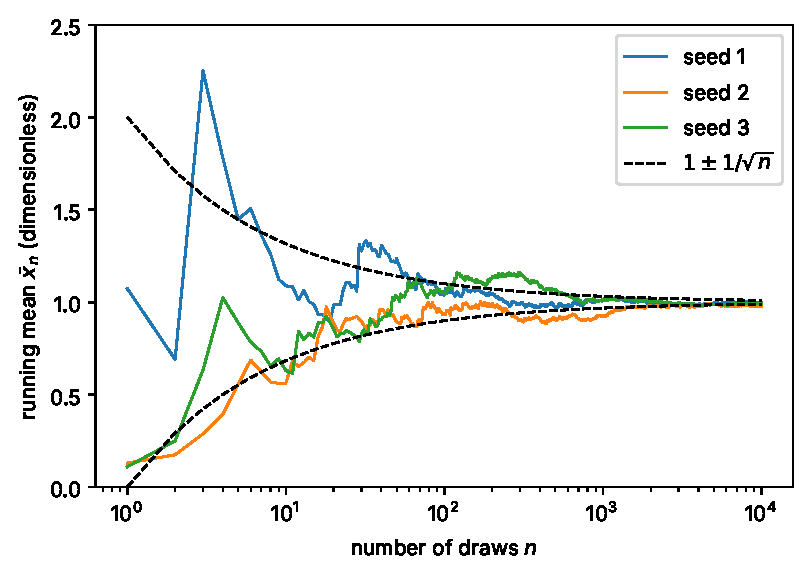
\includegraphics[width=0.85\linewidth]{figs/probability_lln.pdf}
\caption{Law of large numbers. Running sample mean $\bar x_n$ of $n$ exponential draws of mean 1, for seeds 1, 2, 3 of \texttt{numpy.random.default\_rng}. The dashed lines are $1\pm1/\sqrt n$, one standard error \cref{eq:probability-se} either side of the true mean.}
\label{fig:probability-lln}
\end{figure}

\begin{checkpoint}
After $10^4$ exponential draws, is the running mean exactly 1?
\end{checkpoint}
\checkanswer{Almost surely not. The law of large numbers says it is \emph{close} to 1 with high probability; its typical distance from 1 is one standard error, $1/\sqrt{10^4}=0.01$.}

\subsection{Confidence intervals}

\begin{beyond}
\textbf{Taken on trust: the central limit theorem.} If $x_1,\dots,x_n$ are independent and identically distributed with mean $\mu$ and finite variance $\sigma^2$, then for large $n$ the distribution of $(\bar x-\mu)/(\sigma/\sqrt n)$ approaches the standard normal $\varphi$ of \cref{eq:probability-stdnormal}, whatever the distribution of the individual $x_i$. How large $n$ must be depends on the distribution (more for strongly skewed ones). A proof is in \cite{rhb}.
\end{beyond}

Granting the theorem, $\bar x$ lies within $1.96\,\mathrm{SE}$ of $\mu$ with probability about 0.95, by \cref{eq:probability-gauss-table}. Turn the statement around: the interval
\begin{equation}
\bigl[\bar x-1.96\,\mathrm{SE},\ \bar x+1.96\,\mathrm{SE}\bigr]
\label{eq:probability-ci}
\end{equation}
is an approximate \emph{95\% confidence interval} for $\mu$. Its meaning is a statement about the procedure: if you repeated the whole experiment many times and built the interval each time, about 95\% of the intervals would contain the true $\mu$. It is not a statement that $\mu$ ``has a 95\% chance'' of being in your particular interval; $\mu$ is a fixed number, and it either is or is not. For small samples with $\hat\sigma$ in place of $\sigma$, statisticians replace 1.96 by a slightly larger number (from Student's $t$ distribution: 2.06 for $n=25$); we ignore that refinement here.

The paper builds its intervals differently, by the bootstrap (Chapter~\ref{ch:controls}), which does not rely on the central limit theorem but shares the same interpretation.

\begin{sample}{A confidence interval for $g$}
A lab group measures the free-fall acceleration 25 times, getting $\bar x=9.79~\mathrm{m/s^2}$ and $\hat\sigma=0.15~\mathrm{m/s^2}$. Assuming independent measurements, give the standard error and an approximate 95\% confidence interval.

\textbf{Step 1: Standard error.} By \cref{eq:probability-se}, $\mathrm{SE}=0.15/\sqrt{25}=0.03~\mathrm{m/s^2}$.

\textbf{Step 2: Half-width.} $1.96\times0.03=0.0588~\mathrm{m/s^2}$.

\textbf{Step 3: Interval.} By \cref{eq:probability-ci}, $[9.79-0.0588,\ 9.79+0.0588]$.
\[
\boxed{\mathrm{SE}=0.03~\mathrm{m/s^2},\qquad [9.731,\ 9.849]~\mathrm{m/s^2}}
\]
The standard value $9.81~\mathrm{m/s^2}$ lies inside. Notice the distinction: the measurements scatter by $0.15$, but the mean is uncertain by only $0.03$.
\end{sample}

\begin{beyond}
\textbf{Taken on trust: the scatter of a sample correlation.} For $n$ independent pairs from a joint Gaussian distribution with true correlation $\rho$, the sample correlation $r$ has, for large $n$, a standard deviation of approximately $(1-\rho^2)/\sqrt n$. This is a standard normal-theory result, usually derived through Fisher's $z$-transformation; its derivation is beyond this book. A comparison of this normal-theory standard error with bootstrap estimates on a real data set is given in \cite{efron}. Two lessons: correlations near zero are uncertain by about $\pm1/\sqrt n$, and correlations near $\pm1$ are pinned down much more tightly.
\end{beyond}

\begin{keyideas}

\item An estimator is a random variable. $\bar x$ is unbiased with standard error $\sigma/\sqrt n$, \cref{eq:probability-se}, for independent draws.
\item Dividing by $n-1$ makes the variance estimator unbiased (Bessel's correction).
\item Chebyshev's inequality \cref{eq:probability-chebyshev} implies the weak law of large numbers \cref{eq:probability-lln}.
\item With the central limit theorem, $\bar x\pm1.96\,\mathrm{SE}$ is an approximate 95\% confidence interval, \cref{eq:probability-ci}; it describes the long-run behavior of the procedure.

\end{keyideas}

%====================================================================
\section{Random numbers and seeds}\label{sec:probability-rng}

Computers are deterministic machines, so where do the random numbers in \cref{fig:probability-exponential,fig:probability-lln} come from? From a \emph{pseudo-random number generator}: an algorithm that, starting from an internal state, produces a long sequence of numbers that pass statistical tests for randomness (uniform distribution, no detectable correlation between successive values) but is entirely determined by its starting state. The integer that sets the starting state is the \emph{seed}.

Two consequences matter for science. First, \emph{reproducibility}: with the same seed, the same code produces exactly the same ``random'' numbers on every run, so a result that involved randomness can be regenerated digit for digit. Second, \emph{exploring variability}: running with several different seeds shows how much a result depends on the particular random draws.

\begin{pycode}
import numpy as np

rng = np.random.default_rng(1)        # seed 1
a = rng.exponential(1.0, size=5)
rng = np.random.default_rng(1)        # same seed again
b = rng.exponential(1.0, size=5)
print(np.array_equal(a, b))           # True: identical draws

rng2 = np.random.default_rng(2)       # a different seed
print(rng2.exponential(1.0, size=5))  # different numbers

phases = np.random.default_rng(7).uniform(0, 2*np.pi, size=10**5)
print(np.mean(np.cos(phases)), np.mean(np.cos(phases)**2))  # near 0, 0.5
\end{pycode}

The last lines check by simulation two expectations for a uniform random phase $\theta$ on $[0,2\pi)$ with density $1/(2\pi)$:
\[
E[\cos\theta]=\frac1{2\pi}\int_0^{2\pi}\cos\theta\,\dd\theta=\frac{1}{2\pi}\bigl[\sin\theta\bigr]_0^{2\pi}=0,\qquad
E[\cos^2\theta]=\frac1{2\pi}\int_0^{2\pi}\frac{1+\cos2\theta}{2}\,\dd\theta=\frac12 .
\]
These are the facts behind phase randomization: scrambling phases keeps each sinusoid's mean square ($a^2/2$) but destroys its timing.

\begin{pitfall}
Results from different seeds are not independent new data if they all use the \emph{same} underlying data set. Varying the seed of an optimizer, or of a random train/test split drawn from the same zeros, tells you how robust a result is to those random choices. It does not tell you how the result would change on fresh zeros. A range over seeds is therefore not a standard error.
\end{pitfall}

\begin{checkpoint}
A study fits a model ten times with seeds 1--10, always to zeros 1--400, and reports the spread of the ten held-out scores. Does that spread estimate how the score would vary on a new set of zeros?
\end{checkpoint}
\checkanswer{No. All ten runs share the same zeros, so they probe sensitivity to the random choices (initial values, which zeros are held out), not sampling variability of the data. This is exactly the qualification in the caption of the paper's Table~III.}

\begin{keyideas}

\item Pseudo-random generators are deterministic; the seed fixes the whole sequence, which makes random computations reproducible.
\item Different seeds explore the sensitivity of a result to random choices; with fixed data they are not independent samples.

\end{keyideas}

%====================================================================
\section{Paper connection}\label{sec:probability-paper}

We can now read every ``rms / corr'' entry in the paper. First, the quantities being scored.

\paragraph{What is scored.} Recall from Chapter~\ref{ch:counting-zeros} that each zero height $t_n$ has a \emph{smooth position} $s_n$, defined by $\Nsm(s_n)=n-\tfrac12$ with $\Nsm$ the smooth counting function of paper Eq.~(1), and a \emph{local mean spacing} $\gap_n=ds_n/dn$. The fluctuation of zero $n$, in mean spacings, is
\begin{equation}
\delta_n=\frac{t_n-s_n}{\gap_n}.
\label{eq:probability-delta}
\end{equation}
(Here the letter $s$ means smooth zeros, not the spacing variable of \cref{sec:probability-gauss-exp}; the paper uses both, and context tells them apart.) A model that predicts height $\hat t_n$ has predicted fluctuation $\hat\delta_n=(\hat t_n-s_n)/\gap_n$ and error, in spacings,
\[
e_n=\frac{\hat t_n-t_n}{\gap_n}=\hat\delta_n-\delta_n .
\]
The paper's ``rms'' is $\rms(e)$ of \cref{eq:probability-rms} over the scored zeros, and its ``corr'' is the Pearson coefficient \cref{eq:probability-pearson} between $\hat\delta$ and $\delta$ (Sec.~II C: ``reporting rms error in local spacings and the correlation between predicted and true fluctuations''). The \emph{null} predicts $\hat t_n=s_n$, so $\hat\delta_n=0$ and its error is $\rms(\delta)$: the null rms is simply the rms of the true fluctuations. On the principal holdout, zeros 401--500 (Running Example RE5), it is $0.2631$ (Sec.~II C and App.~A, ``Key anchors''), and it grows slowly with height, from $0.263$ to $0.296$ over the holdouts of Table~V. For the fitted potentials the fluctuations are measured relative to the unperturbed potential's levels instead of $s_n$; the paper notes that this null coincides numerically with the smooth-zero null on 401--500, which is what allows one baseline for both comparisons (Sec.~II C). As the pitfall in \cref{sec:probability-corr-rms} explains, the null has no correlation, and indeed none appears in the tables.

\paragraph{Why ``rms worse than the null, corr near zero'' is one fact, not two.} Table~I reports, for the fitted potentials, held-out rms values from $0.265$ to $0.439$ against nulls of $0.261$--$0.274$, with correlations between $-0.17$ and $+0.12$. Sec.~III states that ``the fitted models emit fluctuations of $0.16$--$0.62\times$ the true amplitude that are uncorrelated with truth''. \Cref{eq:probability-uncorr} says that a zero-mean prediction uncorrelated with zero-mean truth has rms $\sqrt{\sigma_y^2+\sigma_p^2}$, always above the null. With $\sigma_y=0.263$ and $\sigma_p$ between $0.16$ and $0.62$ times that, the identity gives $0.266$--$0.309$ (Problem~19): above the null, as every unregularized row of Table~I is. This is a toy reading; actual predictions also have mean offsets, nonzero sample correlations and amplitudes that vary along the holdout, so the table entries are not computed from this formula. It does explain the pattern: a prediction with no correlation cannot beat the null, and the more it fluctuates the worse it does. It also explains the paper's remark that ridge regularization ``moves them smoothly from `memorize more' to `do nothing' and never creates skill'' (Sec.~III): shrinking an uncorrelated prediction lowers $\sigma_p$ toward zero and the rms toward the null, never below it.

\paragraph{The prime formula sits on the optimal-amplitude bound.} The sample problem in \cref{sec:probability-corr-rms} showed that for the zero-parameter formula of paper Eq.~(4), the rms entries of Table~V on 401--500 (0.198, 0.116, 0.074 for 1, 3, 6 primes) match the best rms \cref{eq:probability-bestrms} possible at their correlations (0.198, 0.115, 0.074), under the stated assumption that the true fluctuations have small mean. This is our observation from the paper's numbers, not a claim the paper makes, and the rounding caveat applies near $r=1$.

\paragraph{The arithmetic-continuation probe.} In Sec.~III the paper fits a potential to a synthetic target, the prime-2 wave RE2 (with opposite sign, App.~A step 15) sampled on levels 1--400, and asks it to continue on 401--500. In-sample: rms $0.056$, correlation $+0.95$. Held out: correlation $+0.07$, ``rms worse than predicting zero fluctuation''; App.~A gives the held-out rms $0.1958$ against the probe-null $0.1708$. That probe-null is the rms of RE2 sampled on the holdout, whose long-run value we derived by hand as $0.1709$ in \cref{sec:probability-autocorr}. With the identity \cref{eq:probability-msedecomp} you can even estimate the amplitude the fitted potential emitted on the holdout (Problem~20).

\paragraph{Seeds and ranges.} The paper uses recorded seeds throughout: random restarts of the non-Hermitian fit (App.~A step 10, seed 0), permutations (step 12, seeds 1, 2), random 80/20 splits (step 17, seeds 1--10 and 1, 2), surrogates (step 18, seeds 1--10). The revision computations (steps 16--23) and the permutations of step 12 draw from \texttt{numpy.random.default\_rng(seed)}; for step 10 the paper records the seed 0 without naming the generator. Sec.~II F stresses that every number is regenerated ``deterministically, or from recorded random seeds''. The caption of Table~III states the lesson of \cref{sec:probability-rng} exactly: ``The seeds reuse the same zeros, so the ranges indicate robustness and are not standard errors.'' The caption of Table~I reports optimizer variability the same way: four random-initialization repeats of one configuration gave held-out rms $0.365$--$0.379$.

\paragraph{Intervals.} Sec.~III gives bootstrap 95\% intervals, for example $[0.33,0.43]$ for the held-out rms of the scale-1, $M=400$ random-restart replicate against the null $0.263$, with correlation interval $[-0.21,+0.08]$, and $[+0.95,+0.97]$ for the six-prime formula's correlation on the same holdout. These are confidence intervals in the sense of \cref{sec:probability-sampling}, built by the bootstrap of Chapter~\ref{ch:controls}. Their widths agree in order of magnitude with the Gaussian rule of thumb $(1-\rho^2)/\sqrt n$ of the \texttt{beyond} box on the scatter of a sample correlation in \cref{sec:probability-sampling}: about $\pm0.2$ ($\pm1.96$ standard deviations) near $r=0$, against a half-width of about $0.15$ for the paper's interval $[-0.21,+0.08]$, and about $\pm0.015$ near $r=0.96$ for $n=100$ (Problem~23). Sec.~III (``Other bases'') warns that the intervals in Table~II ``resample held-out levels independently although the fluctuations are serially correlated'', the pitfall of \cref{sec:probability-sampling}; the paper's block-bootstrap recomputation widens them slightly without changing any conclusion (Sec.~III, ``Other bases'').

\paragraph{Autocorrelation and the within-height splits.} Sec.~III (``Within-height splits'') explains the negative held-out correlations of Table~III for $M\le200$: ``the fluctuation sequence has negative autocorrelation at lags 1--3, so any smooth interpolation between neighbouring training levels is anticorrelated with the truth (the mean of the two nearest training fluctuations gives $-0.26$ to $-0.41$).'' \Cref{eq:probability-neighbor} is the simplest version of that mechanism: the neighbor average has the sign of $\rho_1$. Chapter~\ref{ch:generalization} returns to this with the best linear predictor (``kriging''), which the paper reports reaching $0.117$ with correlation $+0.87$ within one height range.

\paragraph{Fig.~2.} The paper's Fig.~2 overlays the Poisson law $e^{-s}$, which we derived in \cref{eq:probability-exponential}, on the unfolded spacings of the first $10^4$ zeros, together with a second curve, the GUE Wigner surmise, which Chapter~\ref{ch:level-statistics} derives. Our \cref{fig:probability-exponential} reproduces the comparison with the Poisson law.

%====================================================================
\section{Summary}
% DYK-BEGIN
\begin{didyouknow}{Random Matrices Began in Statistics}
Random matrices first appeared in statistics, not physics. In 1928 John Wishart derived the distribution of sample covariance matrices built from Gaussian data, now called the Wishart distribution. In the 1950s Eugene Wigner used random matrices to model nuclear energy levels, and in the 1970s they turned up in the Riemann zeros. The same mathematics serves surveys, nuclei and primes.
\end{didyouknow}
% DYK-END

\begin{itemize}
\item A random variable has a discrete distribution $p_j$ or a density $f(x)$; expectations are weighted averages, \cref{eq:probability-mean-discrete,eq:probability-mean-cont}.
\item Variance $\sigma^2=E[(X-\mu)^2]=E[X^2]-\mu^2$, \cref{eq:probability-var,eq:probability-var-shortcut}; $\mathrm{Var}(aX+b)=a^2\sigma^2$, \cref{eq:probability-var-scale}.
\item For a list: mean \cref{eq:probability-sample-mean}, spreads $\sigma_x$ and $\hat\sigma$, \cref{eq:probability-sigma-list,eq:probability-sigma-hat}; rms \cref{eq:probability-rms}; $\rms(e)^2=\bar e^{\,2}+\sigma_e^2$, \cref{eq:probability-rms-bias-spread}.
\item Gaussian \cref{eq:probability-gauss}: mean $\mu$, variance $\sigma^2$; probabilities \cref{eq:probability-gauss-table}.
\item Poisson process: $P(\text{empty interval }s)=e^{-s}$, \cref{eq:probability-empty}; gap density $e^{-s}$ with mean and variance 1, \cref{eq:probability-exponential}.
\item Covariance \cref{eq:probability-cov}; variance of a sum \cref{eq:probability-var-sum}; Pearson $r$ \cref{eq:probability-pearson}; Cauchy--Schwarz \cref{eq:probability-cs} gives $\abs{r}\le1$.
\item Exact link between errors and correlation: \cref{eq:probability-msedecomp}. Uncorrelated predictions lose to the null, \cref{eq:probability-uncorr}; best rms at correlation $r$ is $\sigma_y\sqrt{1-r^2}$, \cref{eq:probability-bestrms}.
\item Autocorrelation \cref{eq:probability-acf}; sinusoids: \cref{eq:probability-sin-acf,eq:probability-sum-ms}; rms of RE2 $=0.1709$; neighbor-average correlation \cref{eq:probability-neighbor}.
\item $\bar x$ is unbiased with $\mathrm{SE}=\sigma/\sqrt n$ for independent draws, \cref{eq:probability-var-mean,eq:probability-se}; Chebyshev \cref{eq:probability-chebyshev} and the weak law \cref{eq:probability-lln}; 95\% intervals \cref{eq:probability-ci}.
\item Seeds make random computations reproducible; ranges over seeds on fixed data measure robustness, not sampling error.
\end{itemize}

%====================================================================
\section{Problems}

\begin{problemlist}
\prob{1}{A fair die is thrown once. What is the probability that the face shown is a prime number?}

\prob{1}{For the list $(2,4,4,4,5,5,7,9)$ find the mean, $\sigma_x$, $\hat\sigma$ and the rms. Check that $\rms^2=\bar x^2+\sigma_x^2$.}

\prob{1}{Two models make errors $(0.2,-0.2,0.2,-0.2)$ and $(0.2,0.2,0.2,0.2)$. Compute the mean, spread $\sigma_e$ and rms of each. What does this tell you about using the rms alone?}

\prob{2}{Prove $\mathrm{Var}(aX+b)=a^2\mathrm{Var}(X)$ starting from the shortcut \cref{eq:probability-var-shortcut} rather than from the definition.}

\prob{1}{For a unit-rate Poisson process, what is the probability that a gap is shorter than half the mean gap?}

\prob{2}{A measured quantity is rounded to the nearest integer. Model the rounding error as uniform on $[-\tfrac12,\tfrac12]$. Find its mean and its rms.}

\prob{1}{Using \cref{eq:probability-gauss-table}, what fraction of a Gaussian distribution lies more than $2\sigma$ from its mean?}

\prob{2}{Compute the Pearson correlation of $x=(1,2,3,4)$ and $y=(2,1,4,3)$.}

\prob{2}{Show that $\corr(ax+b,y)=\corr(x,y)$ for $a>0$ and $=-\corr(x,y)$ for $a<0$, for any constant $b$.}

\prob{2}{Compare the Chebyshev bound for the probability of landing $3\sigma$ or more from the mean with the exact Gaussian value from \cref{eq:probability-gauss-table}.}

\prob{2}{Suppose the fluctuations $\delta_n$ of the zeros on some holdout were Gaussian with mean 0 and standard deviation $0.263$. What fraction would exceed half a mean spacing in magnitude? (Use \texttt{scipy.stats.norm} or a table.)}

\prob{2}{Compute $r_1$ and $r_2$ of \cref{eq:probability-acf} for $x=(1,1,-1,-1,1,1,-1,-1)$.}

\prob{2}{Four hundred independent measurements have $\hat\sigma=0.25$. Find the standard error of their mean and the half-width of an approximate 95\% confidence interval.}

\prob{2}{In a histogram of 1000 numbers with bin width $0.1$, one bin holds 38 entries. What density does \cref{eq:probability-hist-density} assign to that bin?}

\prob{1}{Why does rerunning a numpy program with \texttt{default\_rng(5)} reproduce exactly the same ``random'' numbers?}

\prob{2}{Verify by integration by parts that the exponential density \cref{eq:probability-exponential} has $E[s]=1$ and $E[s^2]=2$.}

\prob{3}{Prove the equality case of Cauchy--Schwarz in detail: if $(\sum u_iv_i)^2=\sum u_i^2\sum v_i^2$ and $\sum v_i^2>0$, then $u_i=\lambda v_i$ for one constant $\lambda$ and all $i$.}

\prob{2}{(Paper.) The caption of Table~III says that the ranges over seeds ``indicate robustness and are not standard errors.'' Explain in your own words why, and say what kind of data would be needed to estimate a genuine standard error of the held-out rms.}

\prob{2}{(Paper.) Sec.~III states that the fitted potentials ``emit fluctuations of $0.16$--$0.62\times$ the true amplitude that are uncorrelated with truth.'' Model truth and prediction as zero-mean with $\sigma_y=0.263$ and $r=0$. Use \cref{eq:probability-uncorr} to find the held-out rms at the two ends of this range, and compare with the null.}

\prob{3}{(Paper.) In the arithmetic-continuation probe (Sec.~III and App.~A), the held-out rms is $0.1958$, the probe-null $0.1708$ and the held-out correlation $+0.07$. Assuming both truth and prediction have zero mean on the holdout, solve \cref{eq:probability-msedecomp} for the spread $\sigma_p$ of the fitted operator's held-out fluctuations, and express it as a fraction of the target's spread.}

\prob{2}{(Paper.) Using \cref{eq:probability-bestrms} with $\sigma_y=0.263$, find the smallest rms possible at correlations $+0.66$, $+0.90$, $+0.96$, and compare with the rms values of the corresponding columns of Table~V on 401--500. State the assumption you need.}

\prob{3}{(Paper.) (a) Using \cref{eq:probability-neighbor}, find the correlation of the neighbor-average predictor when $\rho_1=\rho_2=-0.2$. (b) With $\rho_2=0$, what $\rho_1$ would give $-0.41$, the most negative value quoted in Sec.~III (``Within-height splits'')? (c) Why should the formula be applied to the paper's numbers only as an illustration?}

\prob{2}{(Paper.) Use the rule of thumb $(1-\rho^2)/\sqrt n$ of the \texttt{beyond} box on the scatter of a sample correlation in \cref{sec:probability-sampling} to estimate the standard deviation of the sample correlation of the six-prime formula ($\rho=0.96$) on the $n=100$ held-out zeros 401--500. Form a $\pm1.96$ interval and compare with the paper's bootstrap interval $[+0.95,+0.97]$ (Sec.~III).}

\prob{2}{Using numpy, draw $10^4$ exponential numbers of mean 1 with \texttt{default\_rng(0)}. Compute their mean and variance. Compare the mean with the exact value 1 in units of its standard error; for the variance, just report the relative deviation from the exact value 1.}

\prob{2}{Using qmnt, compute the null rms $\rms(\delta)$ of \cref{eq:probability-delta} on zeros 401--500 and on 501--1000, and compare with the null column of Table~V.}

\prob{3}{Using qmnt, compute the held-out rms and correlation of the one-prime formula, \texttt{qmnt.oracle\_zeros(n, [2])}, on zeros 401--500. Compare with Table~V and with the bound \cref{eq:probability-bestrms} evaluated at your correlation.}

\prob{3}{Using numpy, evaluate RE2 on a fine grid of $t$ covering 1000 periods $2\pi/\log2$ and compute its rms. Compare with the value derived from \cref{eq:probability-sum-ms}.}

\prob{2}{Let $\theta$ be uniform on $[0,2\pi)$, $X=\cos\theta$ and $Y=\sin\theta$. Show that $\mathrm{Cov}(X,Y)=0$ although $X$ and $Y$ are not independent (hint: $X^2+Y^2=1$).}

\prob{3}{Apply Cauchy--Schwarz to the lists $u_i=x_i-\bar x$ for $i=1,\dots,n-k$ and $v_i=x_{i+k}-\bar x$ to prove that $\abs{r_k}\le1$ for the autocorrelation \cref{eq:probability-acf}.}

\prob{2}{For $n=2$ independent throws of a fair die, list or reason over all 36 equally likely pairs to show that $Q=\sum_i(x_i-\bar x)^2$ averages to $35/12$, confirming Bessel's correction.}
\end{problemlist}

%====================================================================
\section{Answers to selected problems}

\textbf{1.} The prime faces are 2, 3, 5. By the addition rule $P=3\times\tfrac16=\tfrac12$.

\textbf{2.} Sum 40, so $\bar x=5$. Deviations $-3,-1,-1,-1,0,0,2,4$; squares sum to 32. $\sigma_x=\sqrt{32/8}=2$; $\hat\sigma=\sqrt{32/7}=2.138$. Mean square $=(4+16+16+16+25+25+49+81)/8=232/8=29$, so $\rms=\sqrt{29}=5.385$. Check: $\bar x^2+\sigma_x^2=25+4=29$. \checkmark

\textbf{3.} First model: mean 0, $\sigma_e=0.2$, rms 0.2. Second: mean 0.2, $\sigma_e=0$, rms 0.2. Both have the same rms, one entirely from scatter and one entirely from bias, \cref{eq:probability-rms-bias-spread}. The rms tells you the size of the errors but not their nature; to diagnose a model you also look at $\bar e$ (or at the correlation).

\textbf{5.} $F(0.5)=1-e^{-0.5}=1-0.606531=0.3935$.

\textbf{7.} $1-0.9545=0.0455$, about 1 in 22.

\textbf{9.} Let $x_i'=ax_i+b$. Then $\overline{x'}=a\bar x+b$, so $x_i'-\overline{x'}=a(x_i-\bar x)$. The numerator of \cref{eq:probability-pearson} is multiplied by $a$; the factor $\sqrt{\sum(x_i'-\overline{x'})^2}=\sqrt{a^2\sum(x_i-\bar x)^2}=\abs{a}\sqrt{\sum(x_i-\bar x)^2}$ is multiplied by $\abs a$. The ratio is multiplied by $a/\abs a=\pm1$.

\textbf{11.} The z-score is $u=0.5/0.263=1.901$. The two-sided tail probability is $2[1-\Phi(1.901)]=0.0573$, where $\Phi$ is the standard normal CDF; about 6\% of the fluctuations. (Whether the real fluctuations are Gaussian is a separate question; \cref{fig:probability-hist_fluct} lets you judge.)

\textbf{13.} $\mathrm{SE}=0.25/\sqrt{400}=0.0125$; half-width $1.96\times0.0125=0.0245$.

\textbf{15.} The generator is a deterministic algorithm. The seed sets its initial internal state, and from a given state every subsequent number is fixed. Same seed, same state, same sequence.

\textbf{17.} Write $S_{uv}=\sum u_iv_i$, $S_{uu}=\sum u_i^2$, $S_{vv}=\sum v_i^2>0$. From the proof of \cref{eq:probability-cs}, with $\lambda^*=S_{uv}/S_{vv}$, $g(\lambda^*)=S_{uu}-S_{uv}^2/S_{vv}$. If $S_{uv}^2=S_{uu}S_{vv}$, this is zero. But $g(\lambda^*)=\sum(u_i-\lambda^*v_i)^2$ is a sum of nonnegative terms; it can vanish only if every term vanishes, so $u_i=\lambda^*v_i$ for all $i$. Conversely, if $u_i=\lambda v_i$, both sides of \cref{eq:probability-cs} equal $\lambda^2S_{vv}^2$.

\textbf{19.} $\rms=0.263\sqrt{1+(\sigma_p/\sigma_y)^2}$. For 0.16: $0.263\sqrt{1.0256}=0.2663$. For 0.62: $0.263\sqrt{1.3844}=0.3094$. Both exceed the null 0.263; uncorrelated output can only add error. The toy model ignores mean offsets and sample correlations, so it is not expected to reproduce Table~I row by row.

\textbf{21.} Assuming the true fluctuations on 401--500 have mean near zero, so $\sigma_y\approx0.263$: bounds $0.263\sqrt{1-r^2}=0.1976$, $0.1146$, $0.0736$, against Table~V's $0.198$, $0.116$, $0.074$. The formula's rms is at the bound to the precision shown, meaning its amplitude is close to the optimal $r\sigma_y$.

\textbf{23.} $(1-0.96^2)/\sqrt{100}=0.0784/10=0.0078$. Then $1.96\times0.0078=0.0154$, giving roughly $[0.945,0.975]$, comparable with the bootstrap $[+0.95,+0.97]$. The rule assumes independent Gaussian pairs, which the serially correlated fluctuations are not, so only the order of magnitude should be compared.

\textbf{25.} About $0.263$ on 401--500 and $0.270$ on 501--1000, matching the null column of Table~V. Code: \texttt{n = np.arange(401, 501); d = qmnt.fluct(qmnt.zeros(1000)[n-1], n); print(qmnt.rms(d))}, and similarly for 501--1000.

\textbf{27.} The rms is $0.1709$, in agreement with $\sqrt{(a_1^2+a_2^2+a_3^2)/2}=0.17088$ from \cref{eq:probability-sum-ms}. Over 1000 whole periods the end corrections are negligible.

\textbf{29.} Let $D=\sum_{i=1}^n(x_i-\bar x)^2>0$. Cauchy--Schwarz \cref{eq:probability-cs} applied to $u_i=x_i-\bar x$ and $v_i=x_{i+k}-\bar x$, $i=1,\dots,n-k$, gives
\[
\Bigl|\sum_{i=1}^{n-k}u_iv_i\Bigr|\le\sqrt{\sum_{i=1}^{n-k}(x_i-\bar x)^2}\,\sqrt{\sum_{i=1}^{n-k}(x_{i+k}-\bar x)^2}.
\]
Each sum under a root contains only some of the nonnegative terms of $D$, so each is at most $D$. Hence the right side is at most $\sqrt D\sqrt D=D$, and dividing by $D$ gives $\abs{r_k}\le1$.
